\chapter{程序模拟结果及对实际机器的模拟研究} \label{chap:Simulation}
随着加速器束流流强的增大,为了对束流进行精确的模拟和研究,我们需要模拟的粒子数目增加了几个量级。
在这种趋势下,束流模拟软件的效率至关重要。
第\ref{chap:Code}章介绍了束流模拟程序在GPU和CPU上的并行实现,
在本章中,小节\ref{section:PIC_performance}和\ref{section:Symplectic_performance}将分别对PIC算法和Symplectic算法的GPU并行性能进行了测试。

之后,我们使用束流模拟软件研究了几个空间电荷相关的问题。
首先,第\ref{section:3rd_order_simulation}节介绍了对空间电荷导致的三阶共振进行的模拟研究,
之后,在第\ref{section:ADS_simulation}节我们使用P-TOPO程序对C-ADS的注入器I进行了模拟研究。

\section{PIC算法性能}             \label{section:PIC_performance}

\subsection{单GPU}
首先,我们通过对比CPU程序和GPU程序的运行速度,来得到GPU程序的的加速比,加速比等于CPU程序耗时除以GPU程序耗时。测试使用的格点数为64*64*64,图\ref{fig:PIC_speedup_1GPU}和表\ref{tab:PIC_speedup_1GPU}是粒子数从16k到1.6m时CPU程序和GPU程序各部分耗时以及加速比。程序消耗的总时间的加速比大约有40,然而每一部分的加速比有很大不同。

其中,橙色柱行代表求解泊松方程,其加速比大约是64,而且并不随粒子数目的变化而变化。事实上,求解泊松方程的计算量主要和格点数相关,而此次测试中我们都是用同样的格点数,因此其耗时基本不变,之后我们会比较在不同格点数情况下求解泊松方程的加速比变化。
灰色柱行代表推动粒子的加速比,其随着粒子数目增加而变大,在粒子数较大时取得超过了70的加速比。
浅蓝色和深蓝色柱行分别是权重差值和粒子信息输出的加速比,其中GPU的权重差值部分包括了粒子排序运算,而且由于其运算的不规则性,加速比较低;而粒子信息输出部分也包含了束团参数的计算,这部分加速比较低是因为输出带宽的限制。


\begin{figure}[!htb]
  \centering
  \begin{tabular}{|l|l|}
    \multicolumn{2}{c}{
    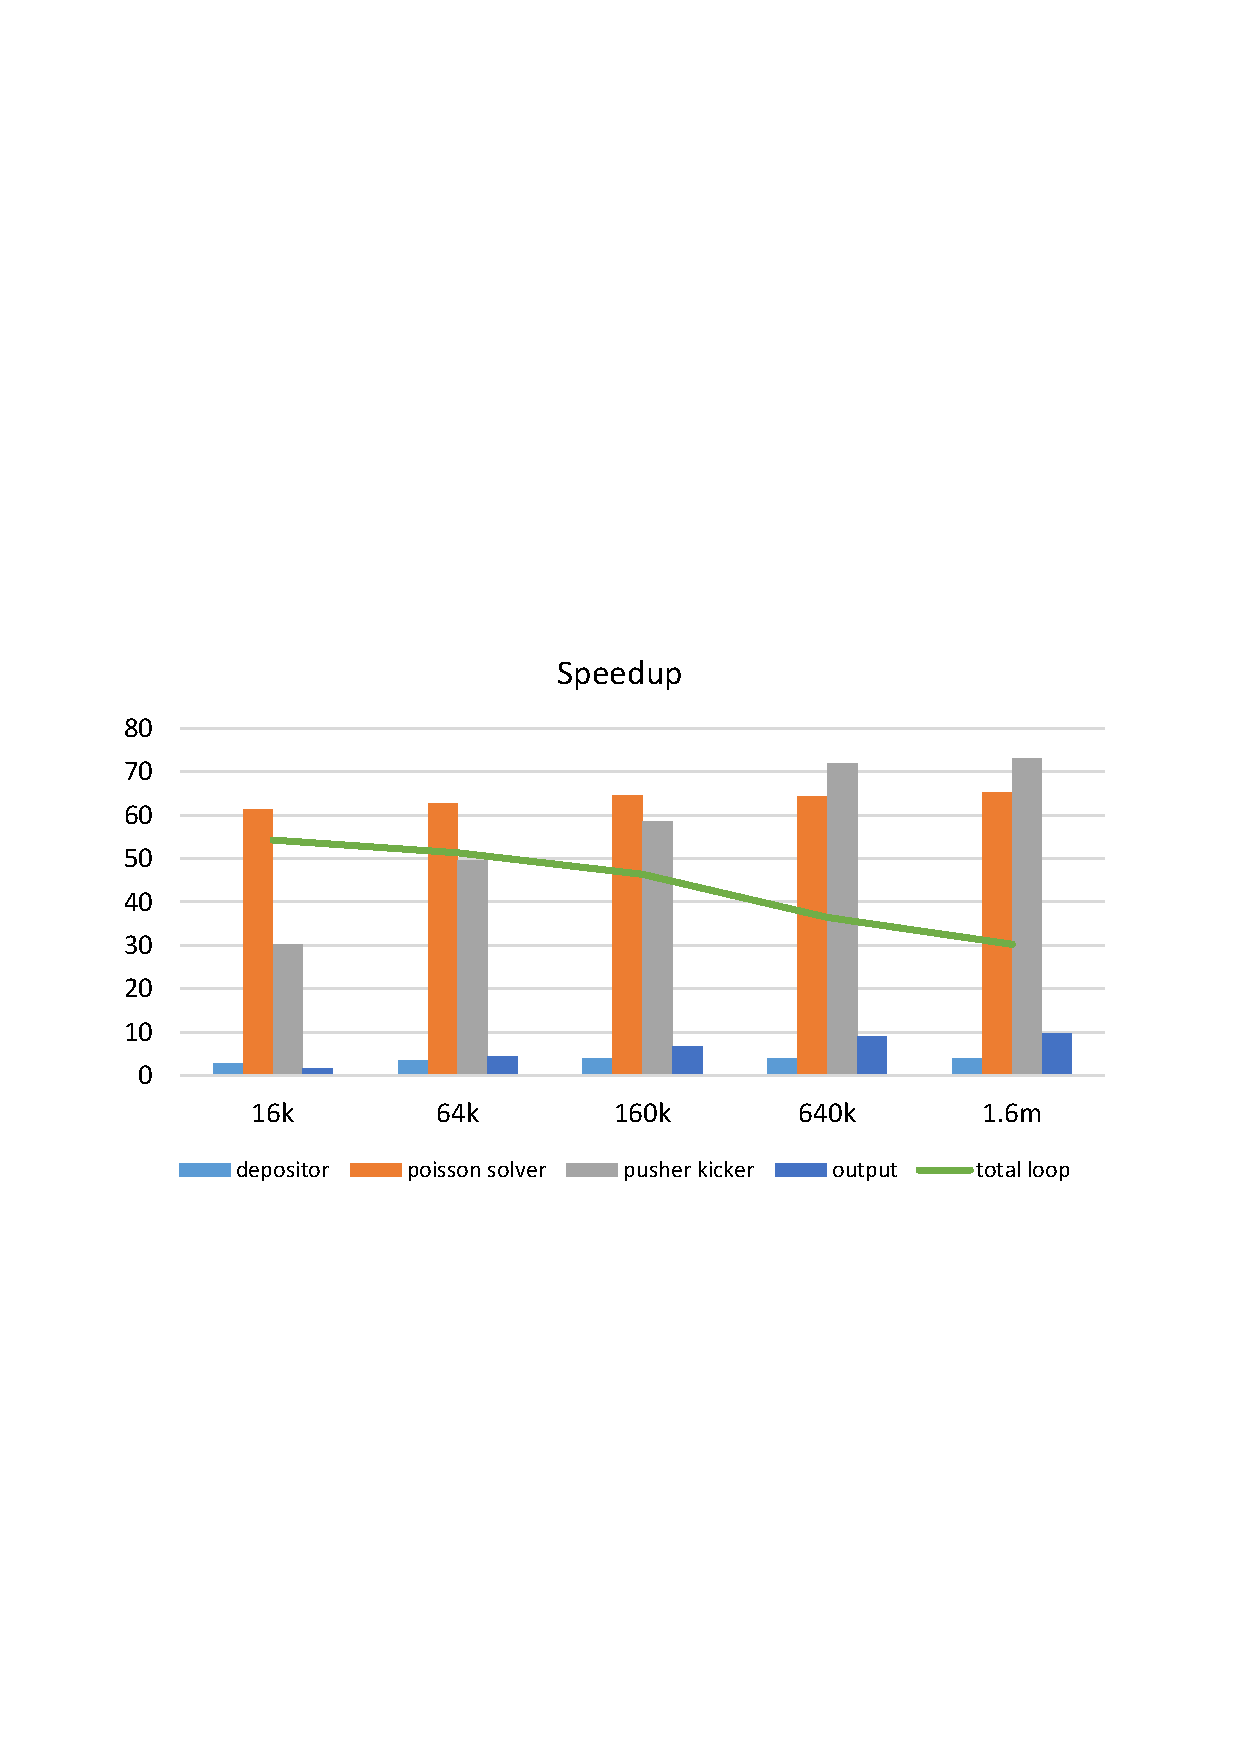
\includegraphics[width=0.9\textwidth]{Img/PIC_speedup_1GPU.pdf}} \\
  \end{tabular}
  \caption{PIC程序在单GPU上的加速比}
  \label{fig:PIC_speedup_1GPU}
\end{figure}

\begin{table}
  \centering
  \begin{tabular}{|l|r|r|r|}
    \hline
    16k                      &    CPU(s)      &     GPU(s)    &  Speedup    \\
    \hline
    depositor (include sort) &    0.16888     &     0.05874   &  2.875043   \\
    Poisson solver           &    26.13173    &     0.42511   &  61.47051   \\
    pusher kicker            &    0.53748	  &     0.01781	  &  30.17855   \\
    output                   &    0.01977     &     0.01149   &  1.720627   \\
    total loop               &    27.78216    &     0.51199   &  54.26309   \\
    \hline
    64k                      &    CPU(s)      &     GPU(s)    &  Speedup    \\
    \hline
    depositor (include sort) &    0.3897      &     0.10847   &  3.592698   \\
    Poisson solver           &    26.08269    &     0.41554   &  62.76818   \\
    pusher kicker            &    2.00422	  &     0.04032	  &  49.70784   \\
    output                   &    0.0641      &     0.01433   &  4.473133   \\
    total loop               &    29.54123    &     0.57598   &  51.28864   \\
    \hline
    160k                     &    CPU(s)      &     GPU(s)    &  Speedup    \\
    \hline
    depositor (include sort) &    0.82705     &     0.20731   &  3.989436   \\
    Poisson solver           &    25.9208     &     0.40208   &  64.46677   \\
    pusher kicker            &    4.88644	  &     0.08343	  &  58.56934   \\
    output                   &    0.15477     &     0.02316   &  6.682642   \\
    total loop               &    32.94187    &     0.71      &  46.397     \\
    \hline
    640k                     &    CPU(s)      &     GPU(s)    &  Speedup    \\
    \hline
    depositor (include sort) &    2.79413     &     0.71529   &  3.90629    \\
    Poisson solver           &    25.72129    &     0.40045   &  64.23097   \\
    pusher kicker            &    22.48269	  &     0.31207	  &  72.04374   \\
    output                   &    0.62289     &     0.06931   &  8.987015   \\
    total loop               &    53.51193    &     1.46745   &  36.46593   \\
    \hline
    1.6m                     &    CPU(s)      &     GPU(s)    &  Speedup    \\
    \hline
    depositor (include sort) &    6.7528      &     1.73779   &  3.885855   \\
    Poisson solver           &    26.03071    &     0.39894   &  65.24969   \\
    pusher kicker            &    56.05512	  &     0.76562	  &  73.21533   \\
    output                   &    1.56528     &     0.16288   &  9.61002    \\
    total loop               &    90.40391    &     2.99053   &  30.23006   \\
    \hline
  \end{tabular}
  \caption{PIC程序在单GPU上的加速比}
  \label{tab:PIC_speedup_1GPU}
\end{table}

权重差值和粒子信息输出的的加速比较低,从而拉低了整体的加速比。整体的加速比随着粒子数的增加而逐渐变小,其原因是当粒子数目较小时的时候,求解泊松方程所占得比重较大,从而整体加速比较大;而当粒子数目变大的时候,权重差值所占的时间比重变大,因而整体加速比随之变小。程序各部分耗时在不同粒子数所占比重如图\ref{PIC_speedup_1GPU_percentage}所示。

\begin{figure}[!htb]
    \centering
    \begin{subfigure}[b]{0.75\textwidth}
        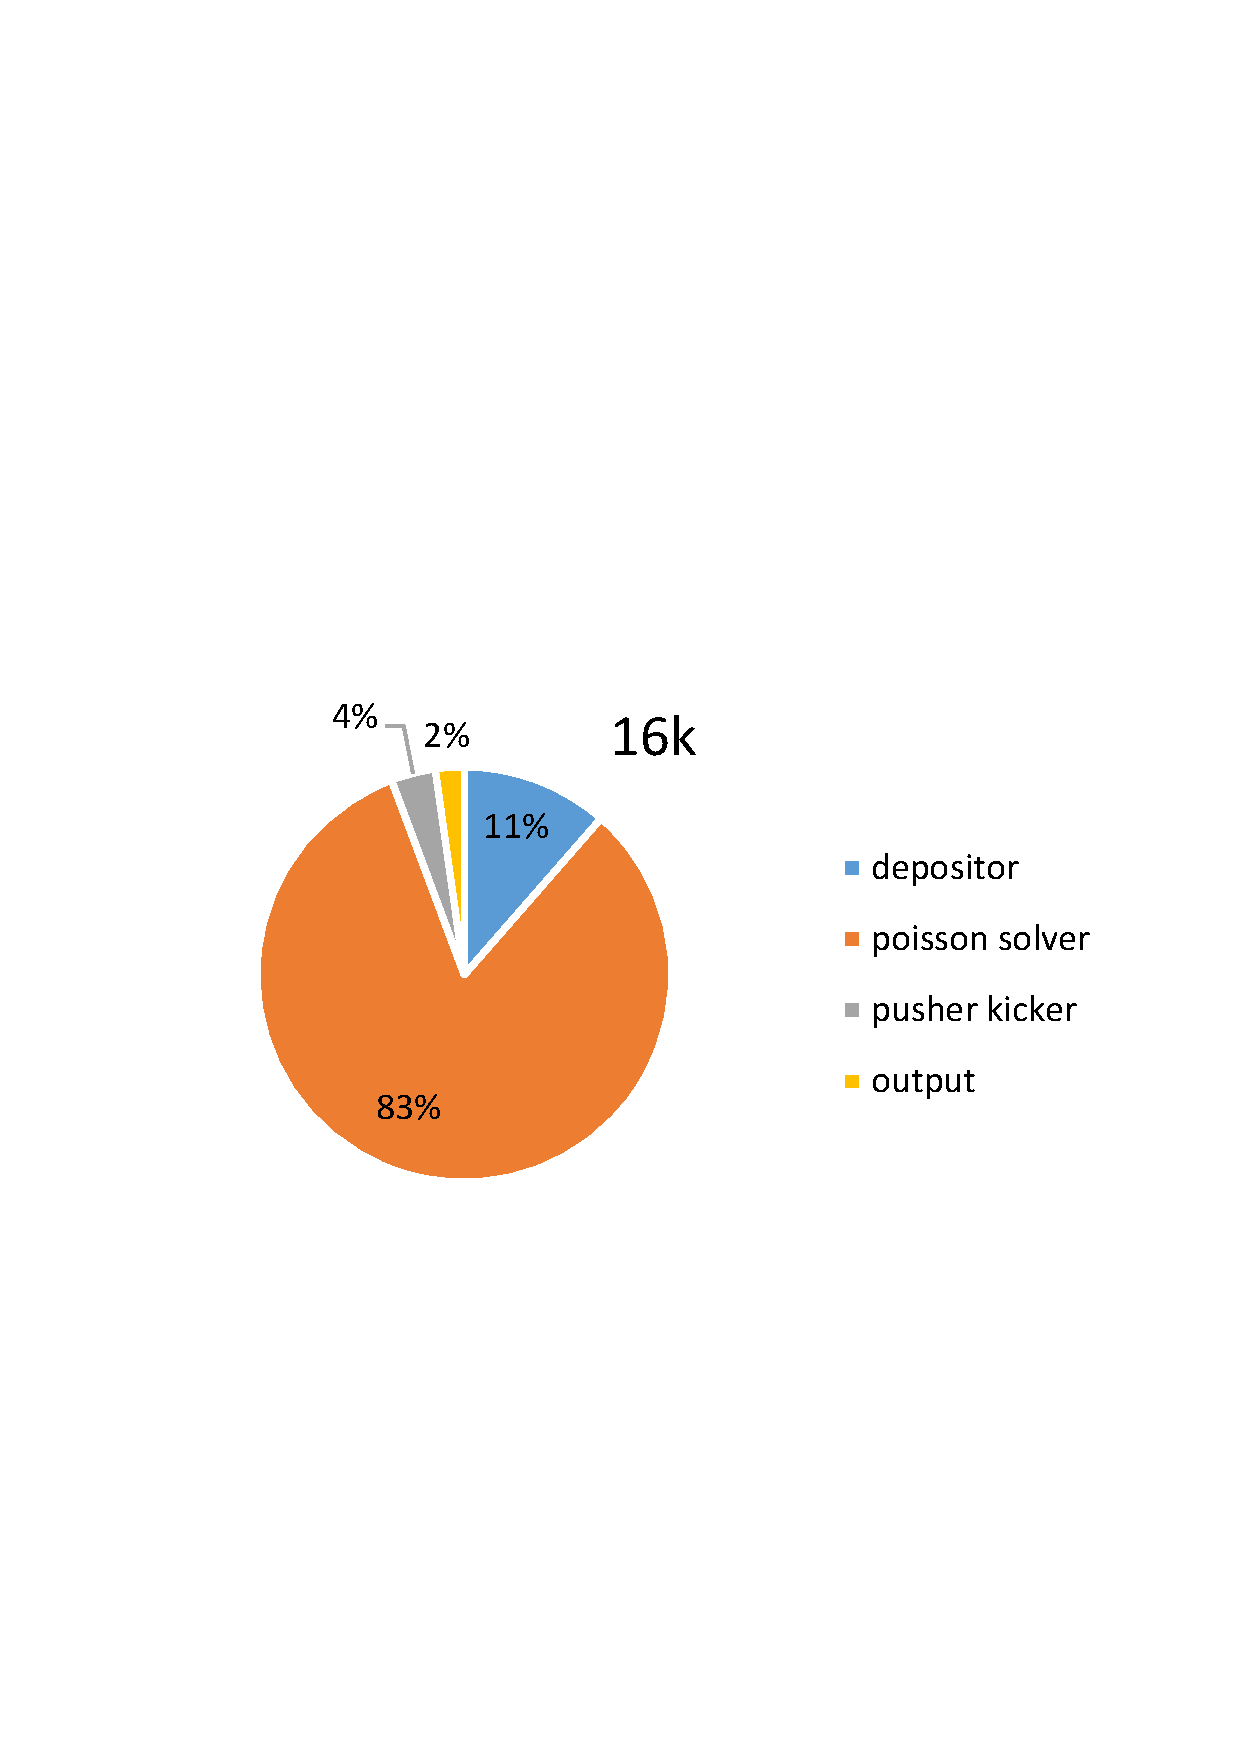
\includegraphics[width=\textwidth]{Img/PIC_speedup_1GPU_percentage1.pdf}
        %\caption{}
    \end{subfigure}
    \quad
    \begin{subfigure}[b]{0.75\textwidth}
        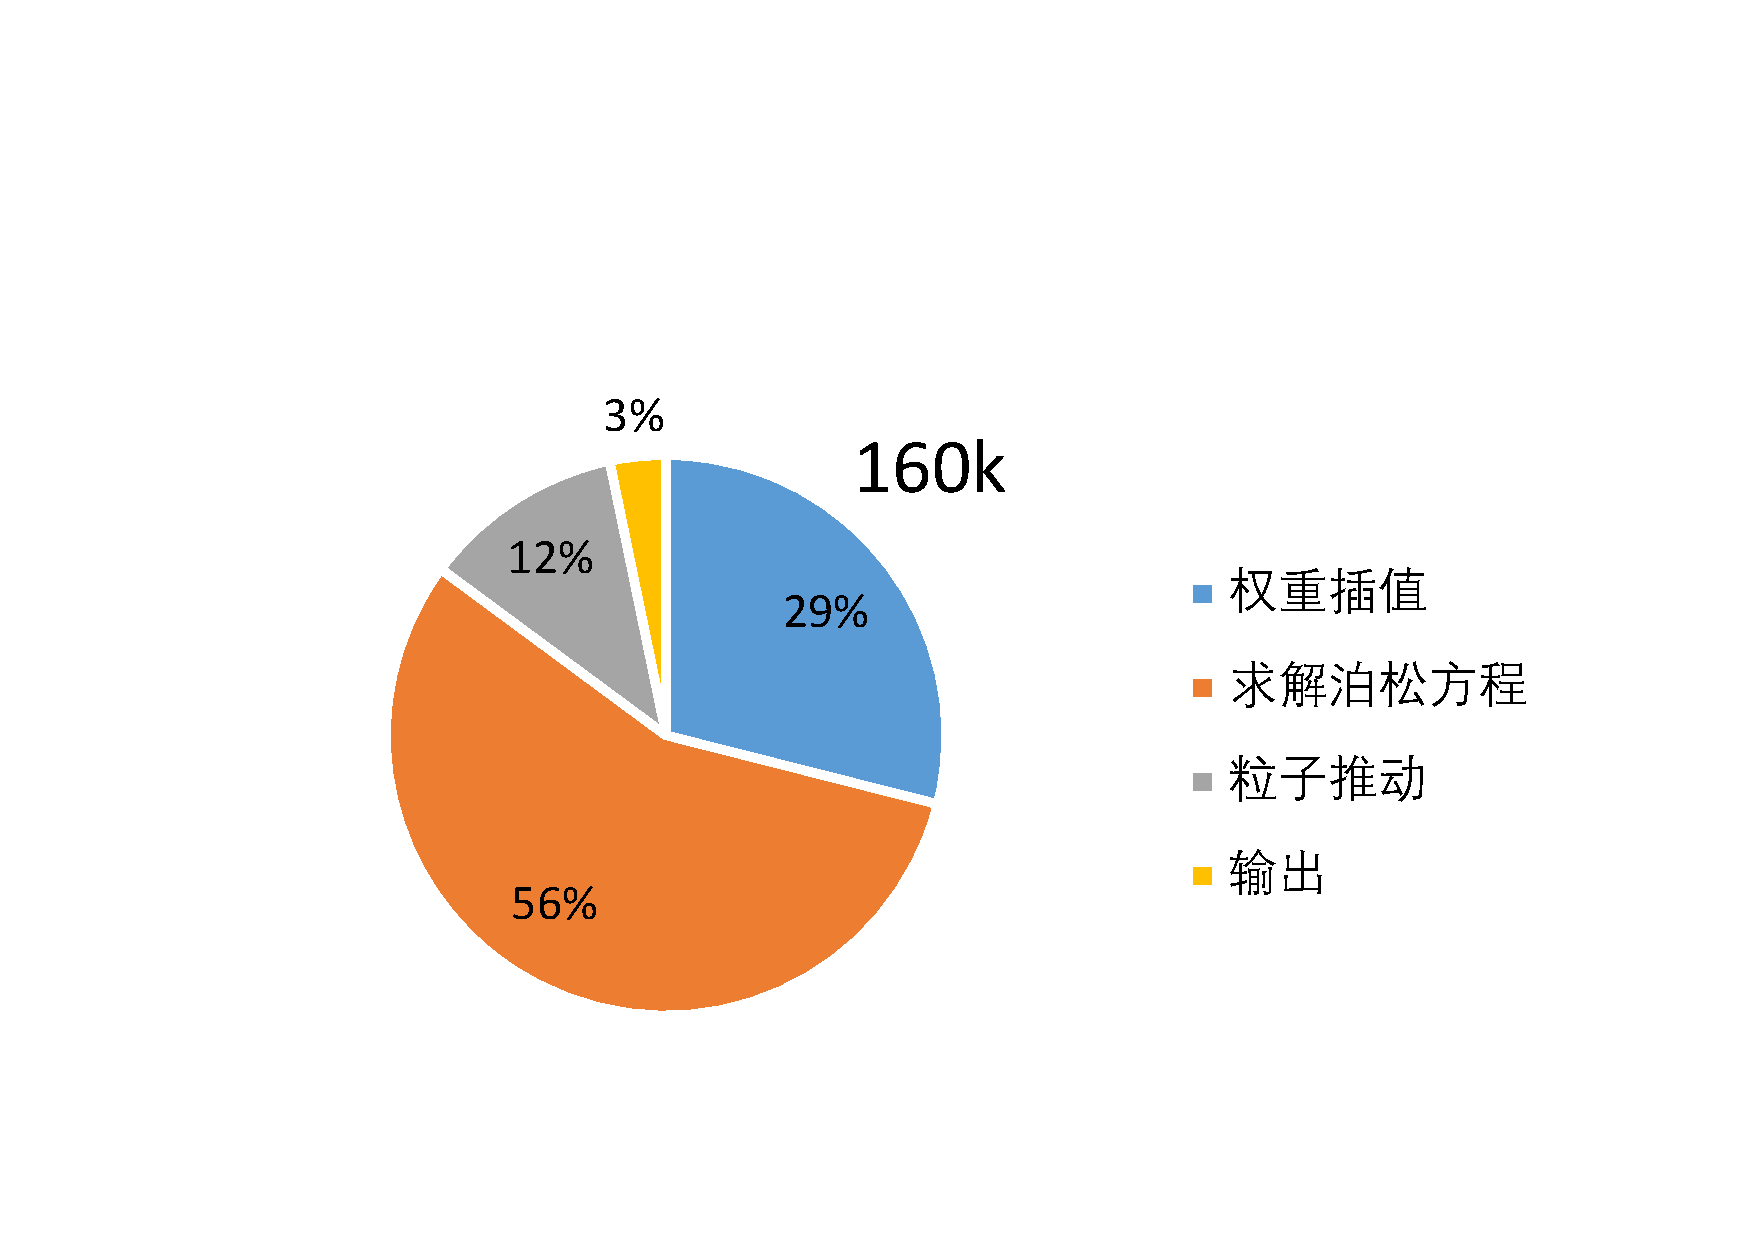
\includegraphics[width=\textwidth]{Img/PIC_speedup_1GPU_percentage2.pdf}
        %\caption{}
    \end{subfigure}
    \quad
    \begin{subfigure}[b]{0.75\textwidth}
        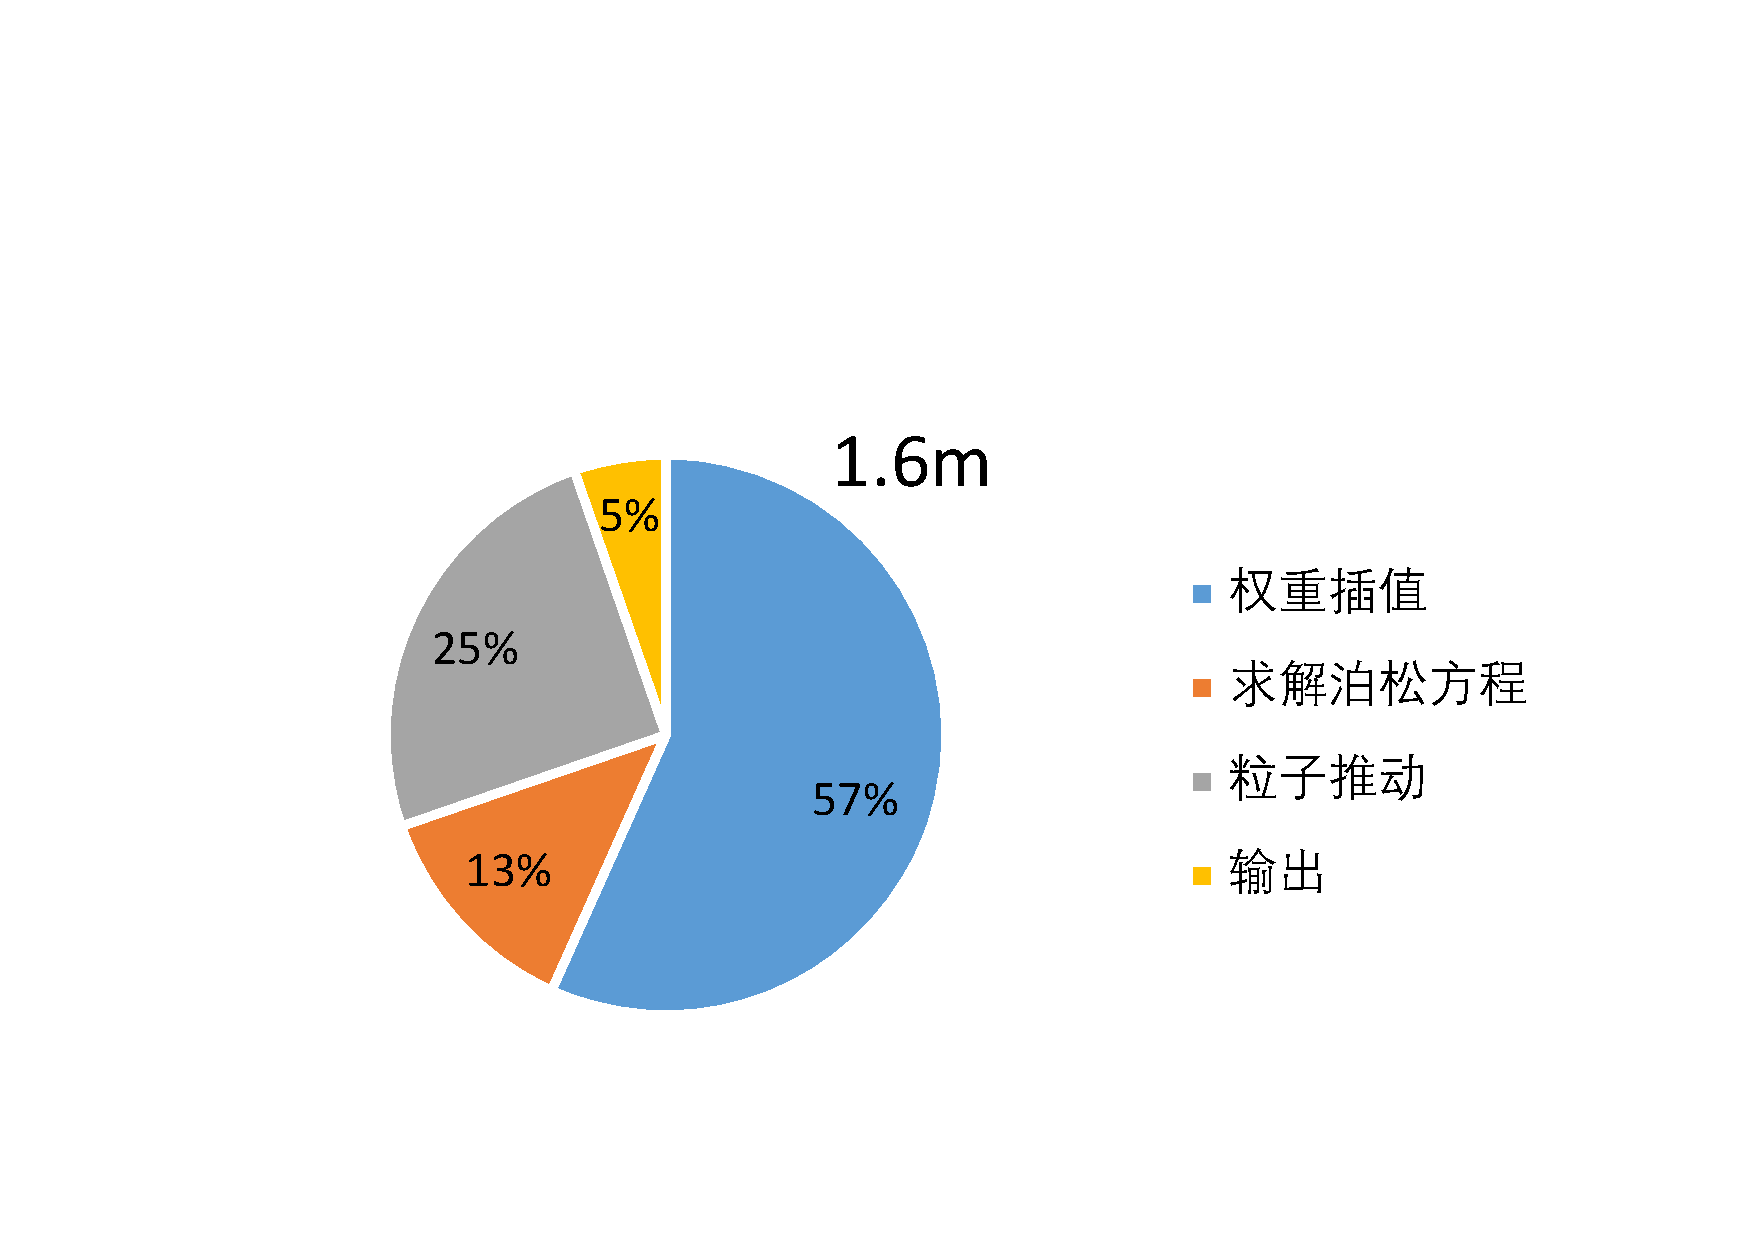
\includegraphics[width=\textwidth]{Img/PIC_speedup_1GPU_percentage3.pdf}
        %\caption{}
    \end{subfigure}
    \caption{程序各部分耗时在不同粒子数时所占百分比}\label{fig:PIC_speedup_1GPU_percentage}
\end{figure}

在上述测试中使用的都是64*64*64个格点数,因此求解泊松方程的时间和加速比都基本不变。在不同的格点数情况下,求解泊松方程的加速比如图\ref{fig:PIC_speedup_1GPU_Poisson}所示。可以看出,求解泊松方程的加速比随着格点数的增加逐渐变大,最终达到了接近70,这是因为格点数越大,其计算量越多,GPU上的负载能够分布得更均匀。在实际模拟中常用的64*64*64个格点和128*128*128个格点中,我们都取得了令人满意的加速比。

\begin{figure}[!htb]
  \centering
  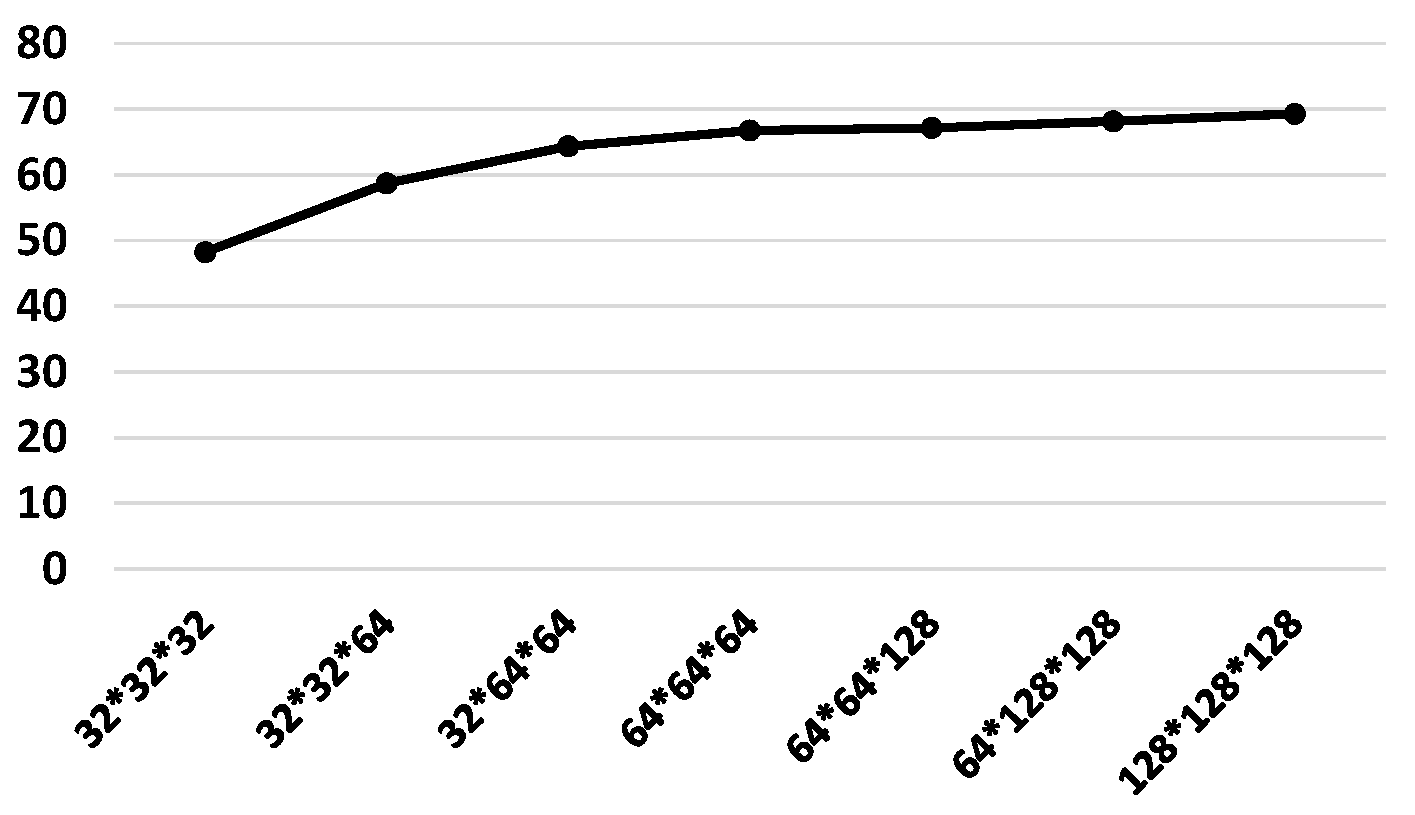
\includegraphics[width=0.9\textwidth]{Img/PIC_speedup_1GPU_Poisson.pdf}
  \caption{不同的格点数情况下单GPU求解泊松方程的加速比}
  \label{fig:PIC_speedup_1GPU_Poisson}
\end{figure}

总之,在单GPU上,程序总体的加速比达到了40,而求解泊松方程的加速比超过到了60,。在一个普通的家用机GPU上运行的速度是在64核机器上运行的两倍。
另外,如小节\ref{section:PIC_GPU_reorder}所述,因为GPU内存大小一般是固定的,而不像CPU内存那样较容易的扩展,所以单GPU的粒子数目存在某个上限,当超过最大粒子数时,应该使用多GPU来进行计算。在接下来的一节中,我们将讨论PIC程序在多GPU上的效率。

\subsection{多GPU}
我们使用超级计算机Titan进行多GPU测试。Titan中每个节点只有一个GPU,型号为NVIDIA K20x,因此只能通过使用多个节点来使用多个GPU。在这种条件下,GPU之间的通讯只能够通过先将数据拷贝到CPU端,再通过CPU端的节点间网络进行通讯。

图\ref{fig:PIC_speedup_Titan_160k_1}为复制模式求解泊松方程时各个部分所花费的时间随GPU个数的变化,可以看出,因为处于复制模式,求解泊松方程的耗时基本保持不变;由于跟多的GPU个数意味着每个GPU上的粒子数随之减小,粒子推动的耗时随着GPU数目的增加而减少;而由于通讯成本随着GPU数目增加而增加,信息统计和输出耗时也随之增加。各个部分对于GPU的数目并不相同,总体来看,总耗时基本保持不变。

\begin{figure}[!htb]
  \centering
  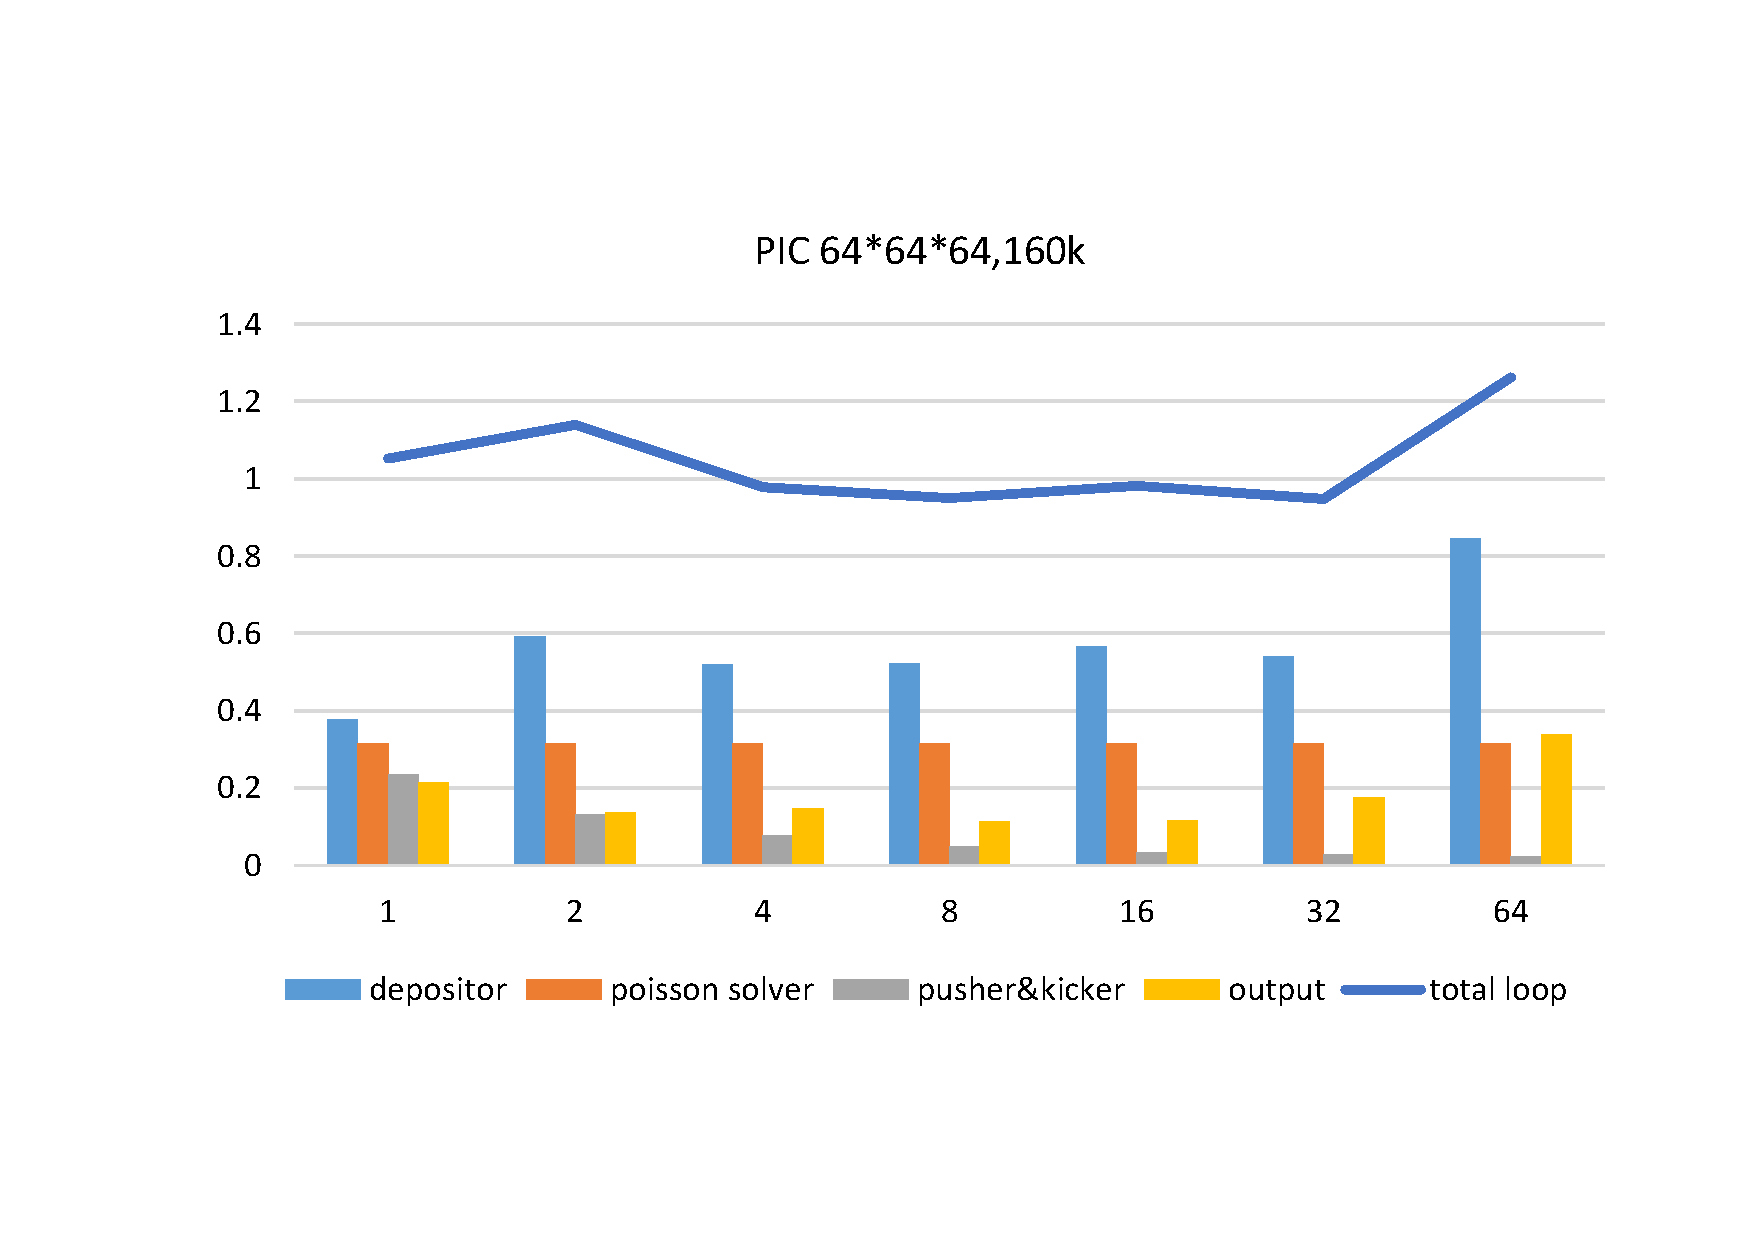
\includegraphics[width=0.9\textwidth]{Img/PIC_speedup_Titan_160k_1.pdf}
  \caption{64*64*64个格点,160k个粒子时,复制模式程序耗时随GPU个数的变化}
  \label{fig:PIC_speedup_Titan_160k_1}
\end{figure}

图\ref{fig:PIC_speedup_Titan_160k_2}和图\ref{fig:PIC_speedup_Titan_160k_1}类似,也是64*64*64各个点,160k个粒子下程序总耗时随着GPU数目的变化。但是在图\ref{fig:PIC_speedup_Titan_160k_2}中,GPU数目大于等于2的时候,求解泊松方程使用域分解模式。其在各种情况下,都相较复制模式耗时更多,主要是拷贝数据花费了大量时间,这个结果和我们在小节\ref{section:PIC_GPU_Poisson}中讨论的相符。因此在之后的测试中,我们都使用复制模式。

\begin{figure}[!htb]
  \centering
  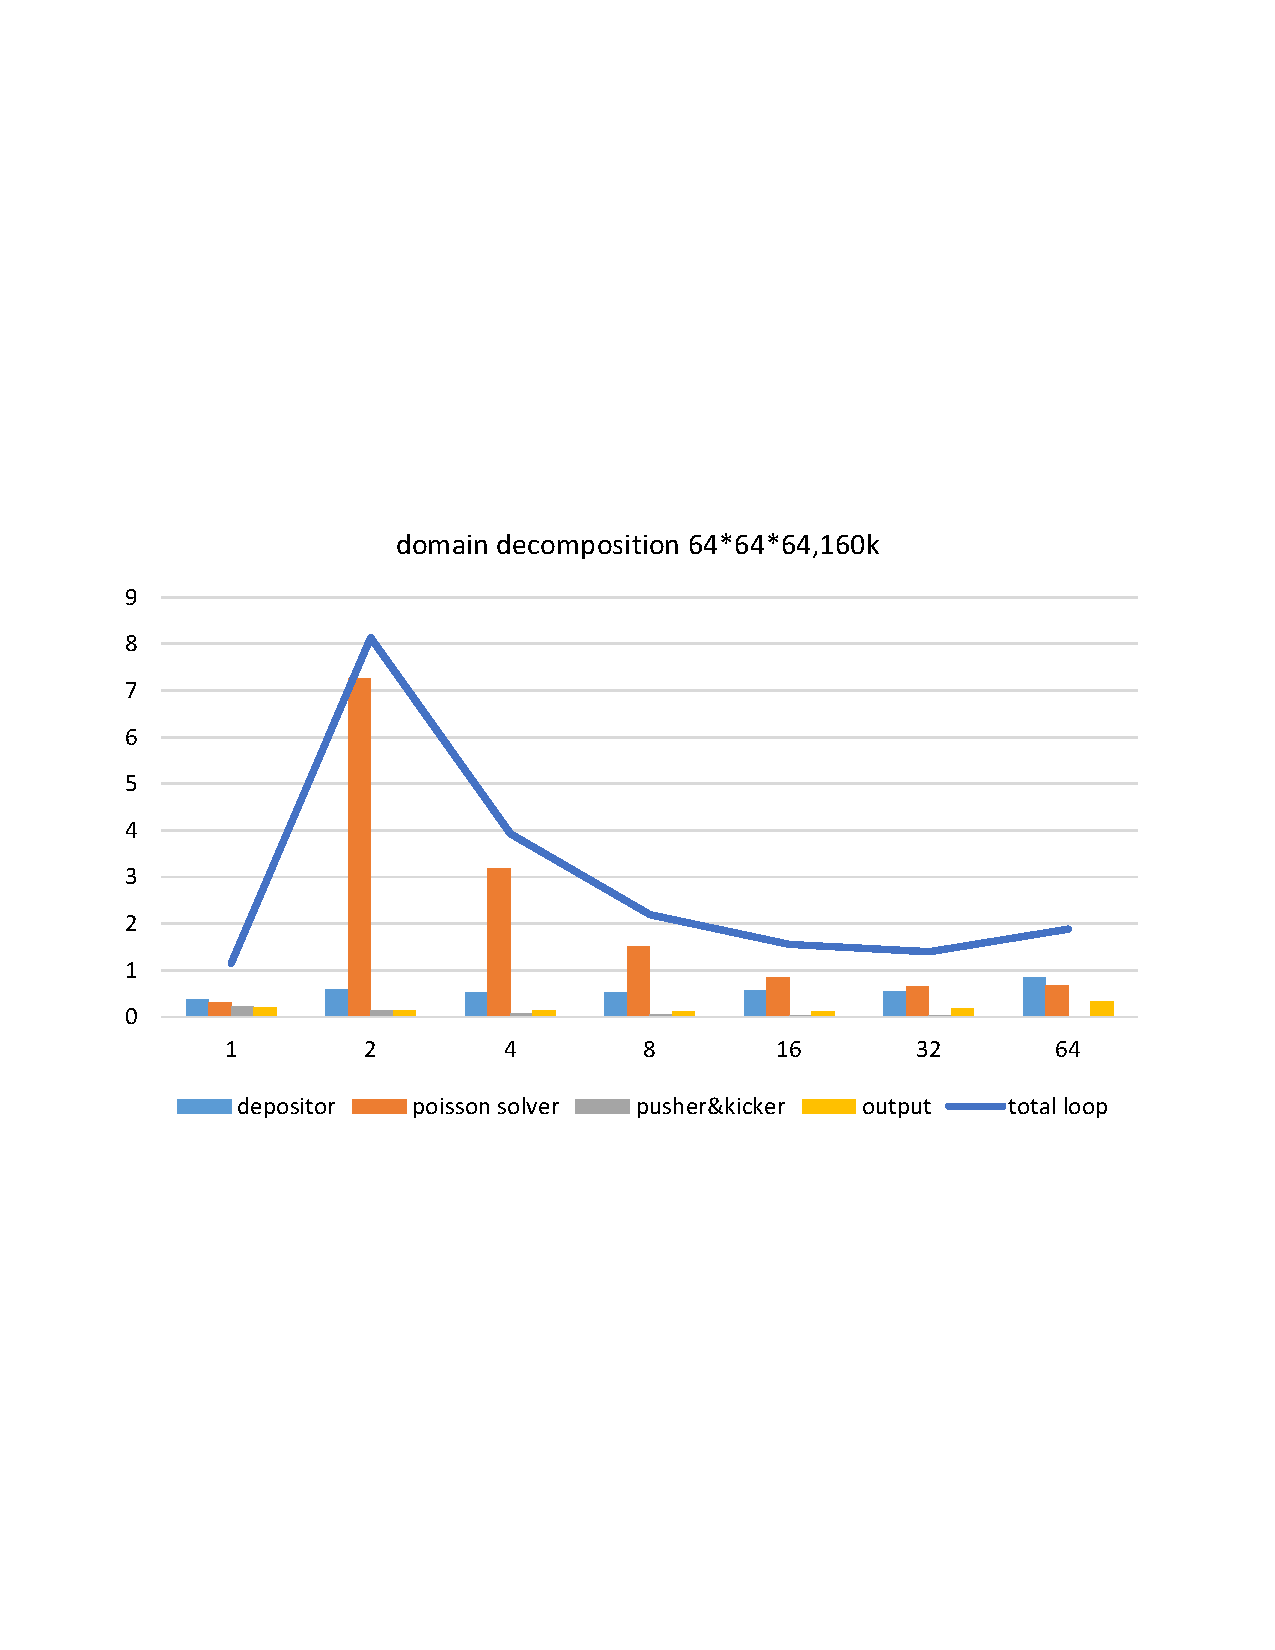
\includegraphics[width=0.9\textwidth]{Img/PIC_speedup_Titan_160k_2.pdf}
  \caption{64*64*64个格点,160k个粒子时,域分解模式程序耗时随GPU个数的变化}
  \label{fig:PIC_speedup_Titan_160k_2}
\end{figure}

当粒子数更大时,耗时的趋势发生了变化。图\ref{fig:PIC_speedup_Titan_1_6m}是粒子数为一百六十万(1.6m)的结果,粒子数较图\ref{fig:PIC_speedup_Titan_160k_1}变大了十倍。在使用1.6m个粒子时,总耗时随着使用的GPU数目增加而明显下降,并在32个GPU处到达最小值。
这是因为在大粒子数目情况下,推动粒子和权重差值所占用的时间占了总时间的绝大部分。而由于使用多GPU带来的每个GPU上的粒子数目变少,推动粒子和权重差值能够很好的被多GPU加速。

\begin{figure}[!htb]
  \centering
  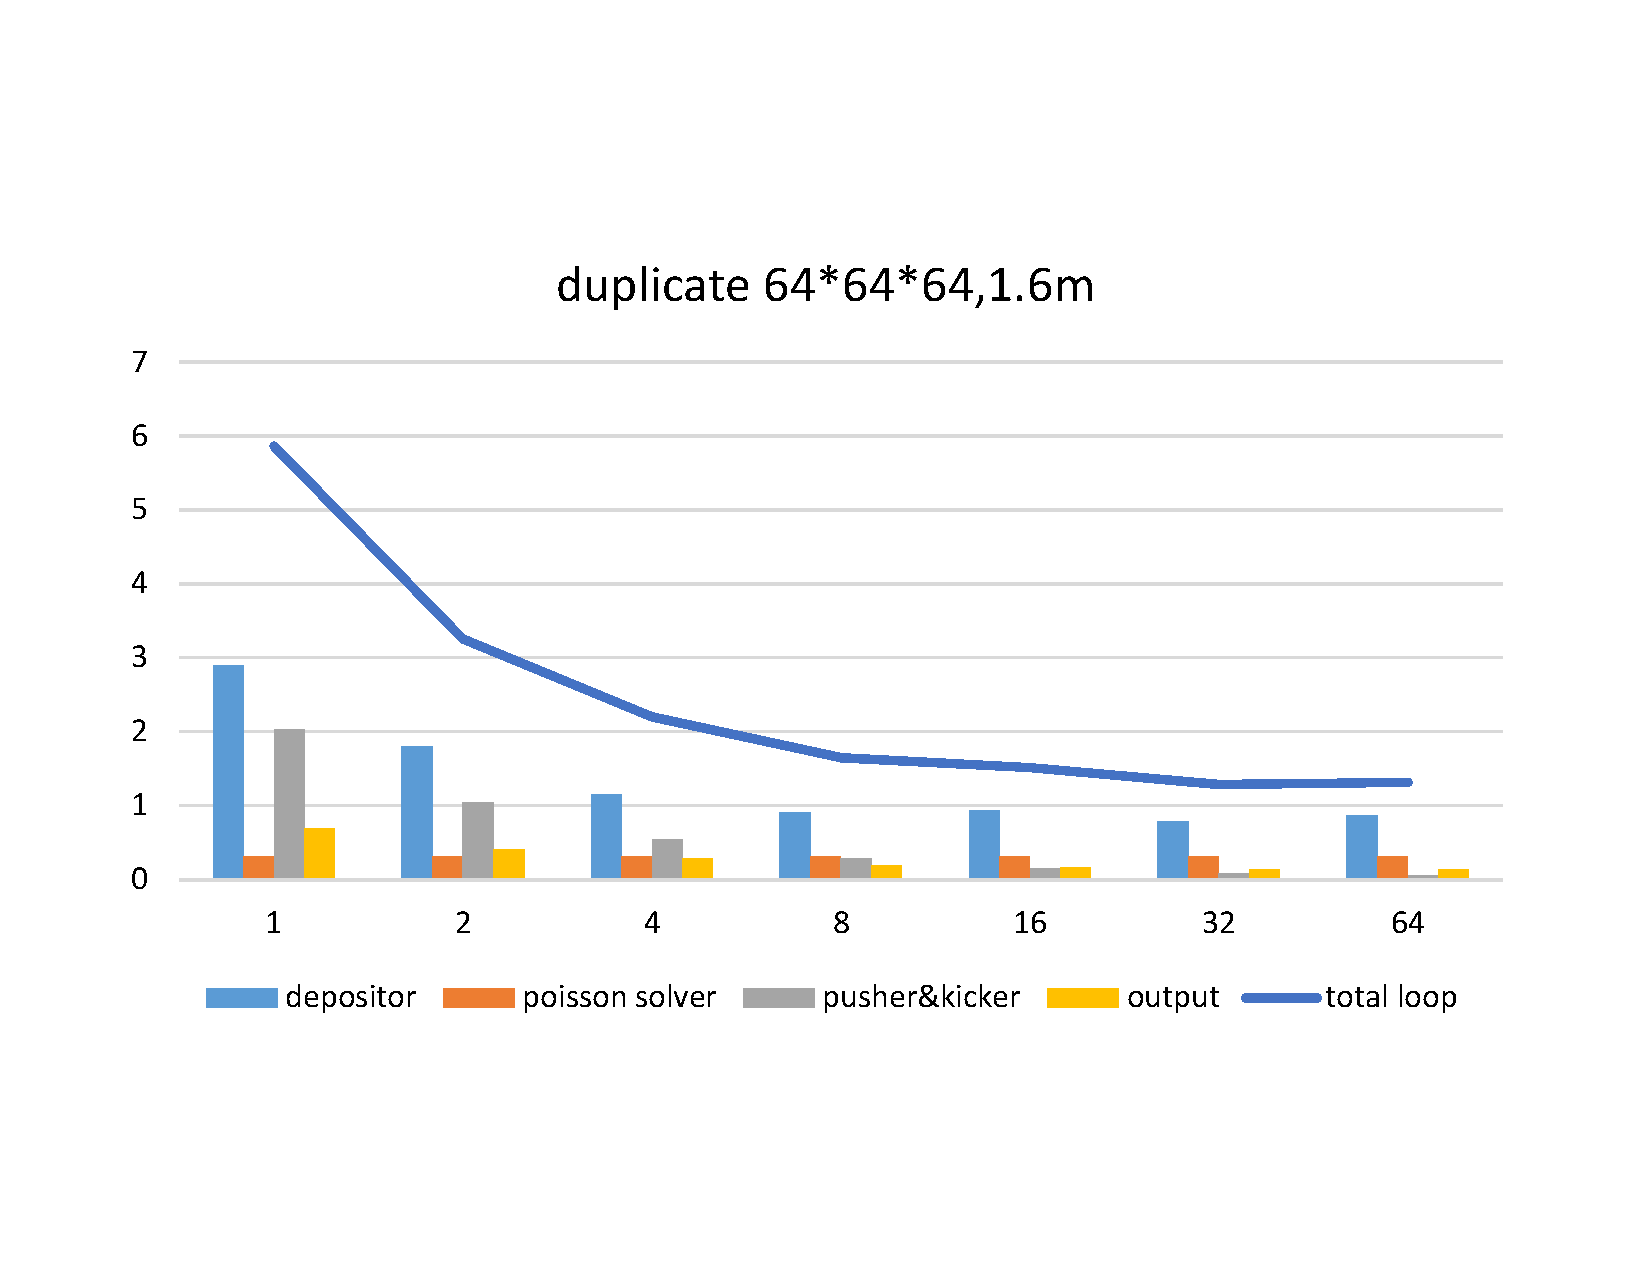
\includegraphics[width=0.9\textwidth]{Img/PIC_speedup_Titan_1_6m.pdf}
  \caption{64*64*64个格点,1.6m个粒子时,程序耗时随GPU个数的变化}
  \label{fig:PIC_speedup_Titan_1_6m}
\end{figure}

我们尝试使用更大的粒子数,一千六百万个粒子(16m),更十倍于前,如图\ref{fig:PIC_speedup_Titan_16m}所示。由于GPU内存大小的限制,程序在这个粒子数下不能仅仅使用1或2个GPU运行,因此在图\ref{fig:PIC_speedup_Titan_16m}中,GPU数目等于1和等于2的时候没有数据。

超级计算机Titan上使用的GPU型号为NVIDIA K20x,每个GPU有5GB的内存。理想情况下,一个5GB内存能够使用的最大粒子数为六千万(60m)。但这个粒子数是在空间均匀分布下才能使用,而实际上,我们很难达到这个粒子数。一个实际的加速器模拟中我们通常使用KV,WaterBag,或者高斯分布,因此其可用的粒子数目远小于理想数目。

\begin{figure}[!htb]
  \centering
  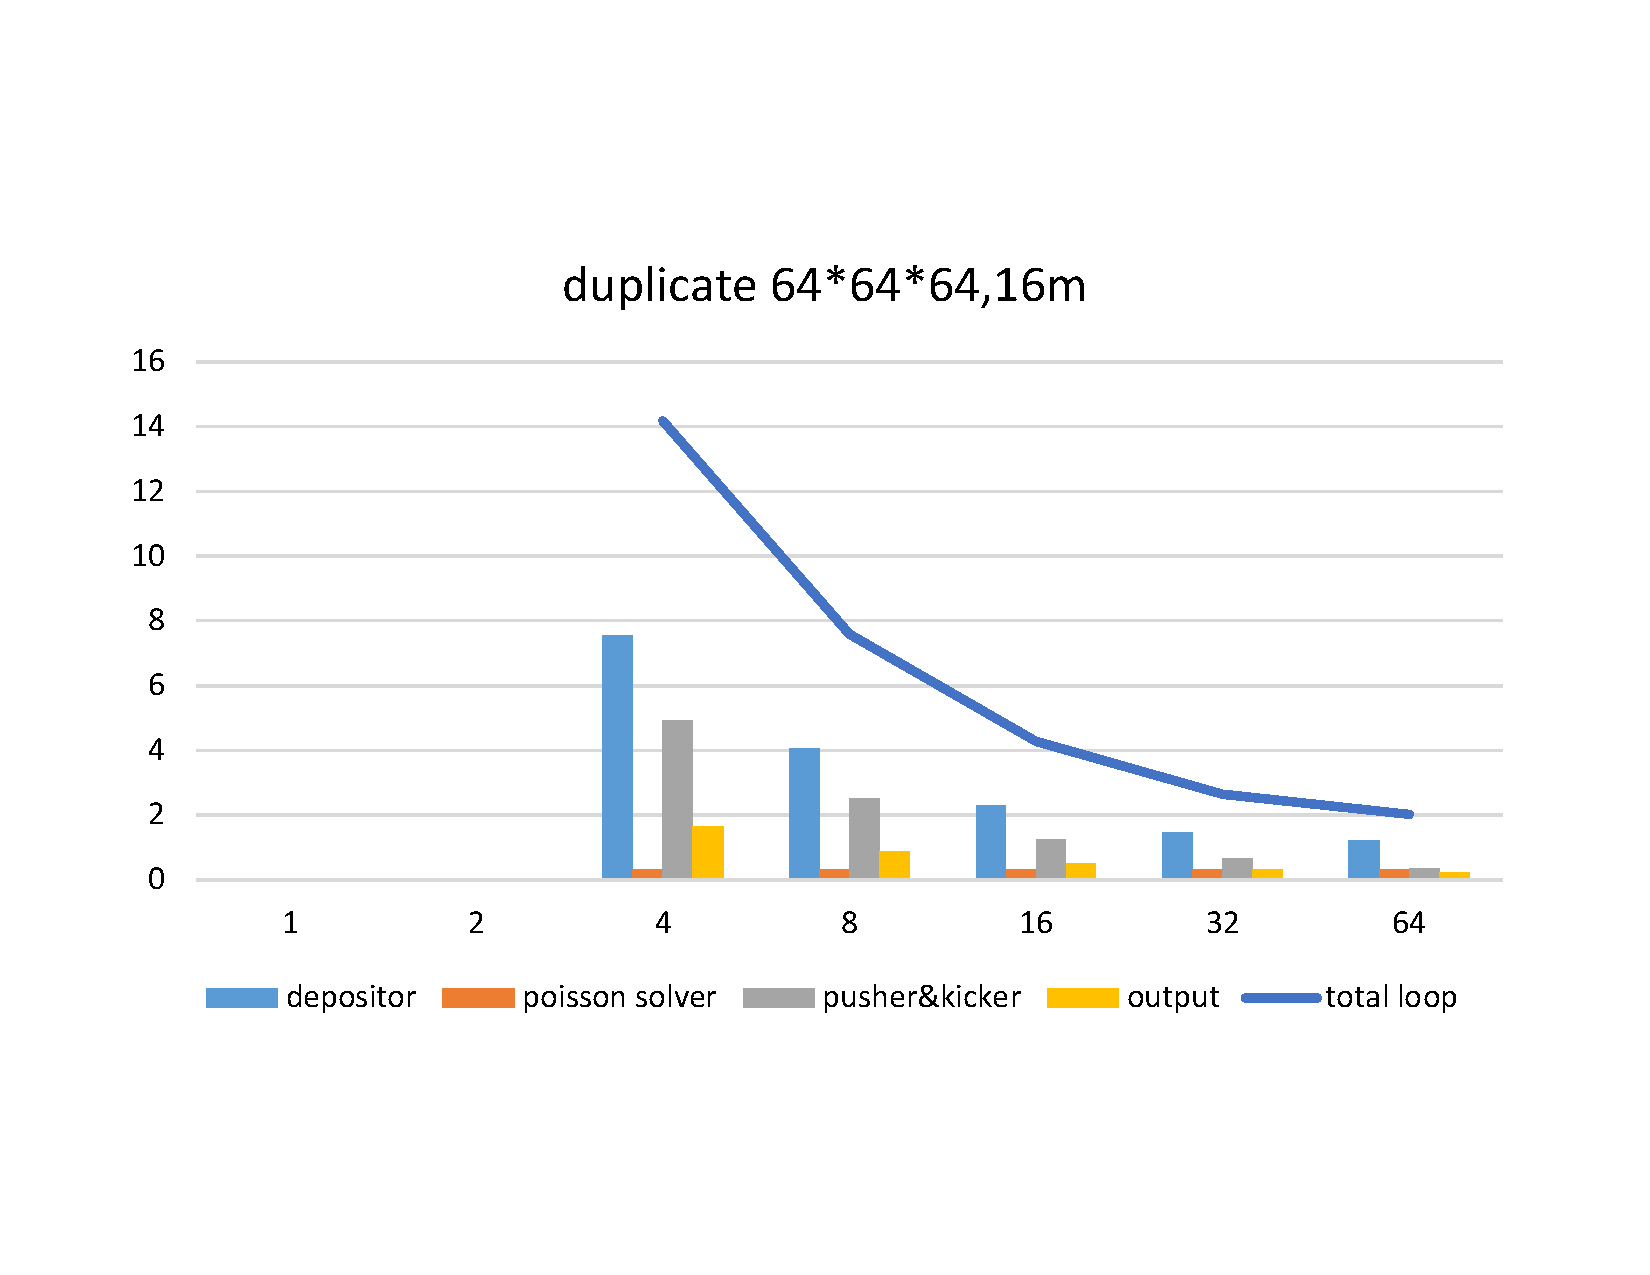
\includegraphics[width=0.9\textwidth]{Img/PIC_speedup_Titan_16m.pdf}
  \caption{64*64*64个格点,16m个粒子时,程序耗时随GPU个数的变化}
  \label{fig:PIC_speedup_Titan_16m}
\end{figure}

\section{Symplectic算法性能}      \label{section:Symplectic_performance}
我们使用GPU程序的性能和可拓展性进行了两个测试,第一个测试使用一个普通的家用GPU:GTX 1060 6GB,测试的结果与在CPU串行运行的程序进行比较。第二个测试使用美国能源部下属的橡树岭国家实验室(ORNL)的GPU集群泰坦,用于测试程序的可扩展性,即程序在多GPU下的表现。

\subsection{单GPU性能提升-GTX1060}
首先,我们将GPU代码的性能与CPU代码进行比较。GPU代码使用GeForce GTX 1060 6GB(Pascal架构)进行测试,而作为对比的CPU代码使用AMD Opteron(tm)6134的一个核心运行,测试的软件环境为Ubuntu 16.04,使用CUDA 8.0版。

加速比由CPU版本运行的运行时间,除以GPU版本的运行时间得到。在本次测试中,我们对空间电荷求解器和整个程序分别进行了比较。空间电荷求解器包括将数据从CPU侧复制到GPU侧,计算空间电荷效应,推动粒子,并将数据复制回CPU侧,而整个程序则包括了除了空间电荷求解器之外的所有其他部分,比如外场推动,输入,统计,输出等等。

从CPU代码简单的移植到GPU代码就可以实现大约200倍的加速,但是我们通过优化可以获得更大的加速比。
在采用了小节\ref{section:symplectic_GPU}中的优化策略后,程序能够充分利用GPU,取得了超过400的加速比。
接下来,如图\ref{fig:OneGPU}所示,我们会讨论分别讨论空间电荷效应和整个程序在不同的问题规模大小下的加速比。

\begin{figure}[!htb]
    \centering
    \begin{subfigure}[b]{0.9\textwidth}
        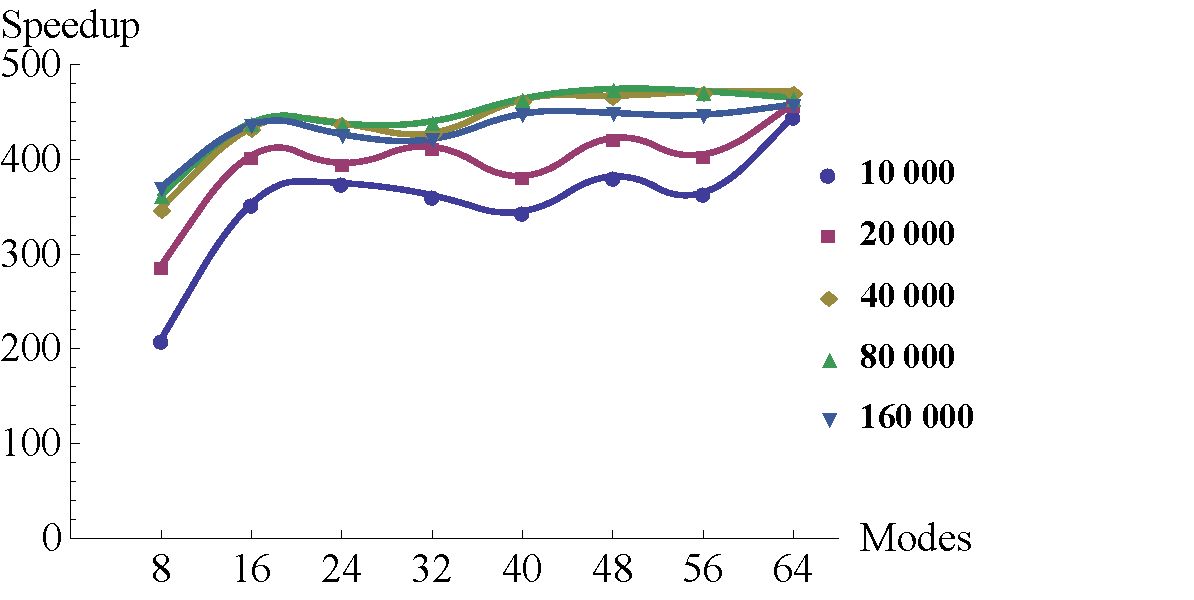
\includegraphics[width=\textwidth]{plot/SpaceChargeGPU11th_large.pdf}
        \caption{空间电荷效应求解器加速比}
        \label{fig:SCOpt}
    \end{subfigure}
    \quad
    ~ %add desired spacing between images, e. g. ~, \quad, \qquad, \hfill etc.
      %(or a blank line to force the subfigure onto a new line)
    \begin{subfigure}[b]{0.9\textwidth}
        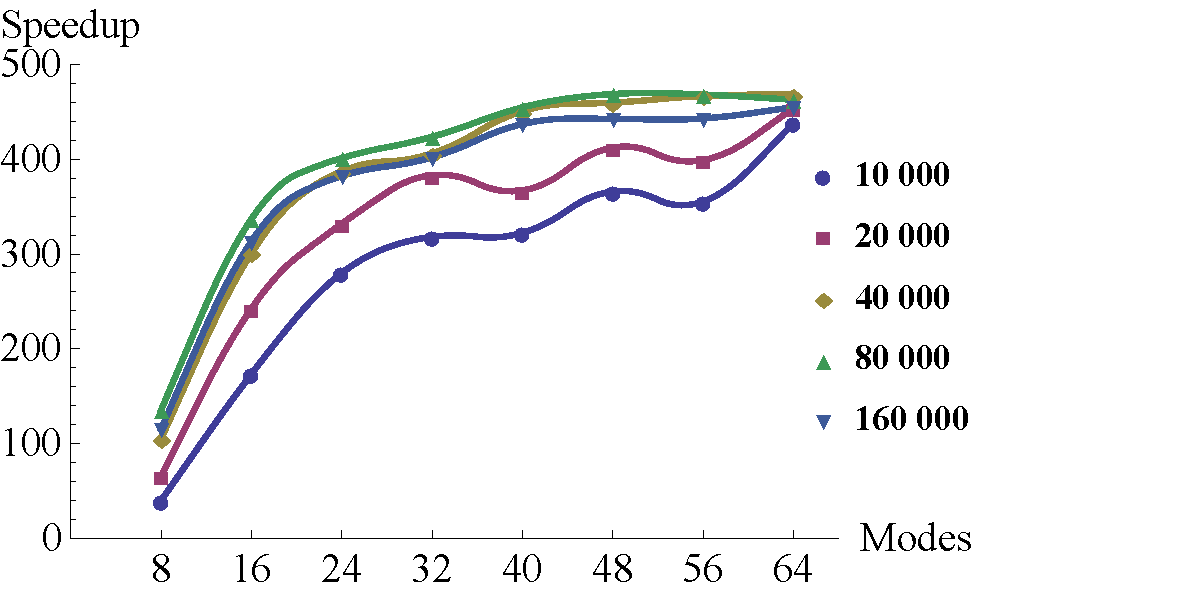
\includegraphics[width=\textwidth]{plot/TotalGPU11th_large.pdf}
        \caption{程序整体加速比}
        \label{fig:TotalOpt}
    \end{subfigure}
    \caption{单GPU加速比}\label{fig:OneGPU}
\end{figure}

图\ref{fig:SCOpt}为优化后的空间电荷效应求解器的加速比在不同的问题规模下的变化。其中,横坐标为展开的阶数,而纵坐标是加速比,不同的线是不同粒子数目的结果。可以看到,阶数越大加速比越高,这与我们的预期符合,因为阶数越大意味着空间电荷求解器占用的时间在总时间中的比例越大。其中,在$8*8*8$阶时加速比很低,因为在这种模式下的计算量很低。随着阶数的增加,计算量也随之增加,GPU的负载更为平衡,因此取得了更大的加速比。另一方面,粒子数目对于加速比的影响很小,在大阶数的情况下尤为如此。这是因为粒子数目本身远远超出了一个GPU的核心数目(在GTX 1060 上为1280个核心),即时在最低粒子数(10000个粒子)的情况,程序也能有效的使用所有的核心,而随着粒子数目的轻微提升是因为GPU能够在更大运算量的情况下更好的协调和平衡计算资源。

图\ref{fig:TotalOpt}为程序整体的运行时间的加速比,除了空间电荷效应求解之外,程序总体运行时间还包括外部传输矩阵,从Z坐标到T坐标的变换,粒子信息统计以及输入输出。
同空间电荷效应求解器相比,整体时间的加速比在各个问题规模下都略有下降,但是加速比变化的趋势却保持一致。
其中,在低阶情况下,比如$8\times8\times8$阶或$16\times16\times16$阶,因为空间电荷效应求解器所占总时间的比重不大,所以加速比的下降更为严重。
然而,在高阶情况下,空间电荷效应求解所占的时间会占总时间的绝大部分,所以总时间的加速比和空间电荷效应求解的加速比能够基本保持一致。

总之,我们取得了非常好的加速比。对于程序整体的总运行时间,优化的GPU代码比CPU代码运行速度高450倍;而如果仅仅比较空间电荷效应求解器,其最大加速比超过了460。

\subsection{多GPU性能提升-泰坦}
泰坦使用CPU和GPU混合架构,是目前世界上最快,规模最大的计算机集群之一。泰坦的每个节点拥有一个AMD Opteron(16核心)的CPU和一个NVIDIA Tesla K20x (2688核心)的GPU。为了测试多GPU的程序可扩展性,我们最多使用了1024个节点进行测试。其中,为了在不同节点的GPU上交换信息,我们需要先把GPU上的数据拷贝到CPU侧,再使用MPI协议在不用节点之间交换数据,最后再将交换后的信息拷贝回GPU侧。
在本次测试中,我们使用16$\times$16$\times$16阶进行测试,使用这个阶数是为了精确度和计算速度之间的平衡,也是我们在实际模拟中最常用的阶数。
如图\ref{fig:Titan}所示,我们分别讨论了空间电荷效应和整个程序在不同的粒子数目下,在不同的节点数上的加速比。其中,横轴为节点数目,纵周围加速比,加速比有多节点的运行时间除以单节点的运行时间得到,不同线是不同粒子数目的结果。

\begin{figure}[!htb]
    \centering
    \begin{subfigure}[b]{0.9\textwidth}
        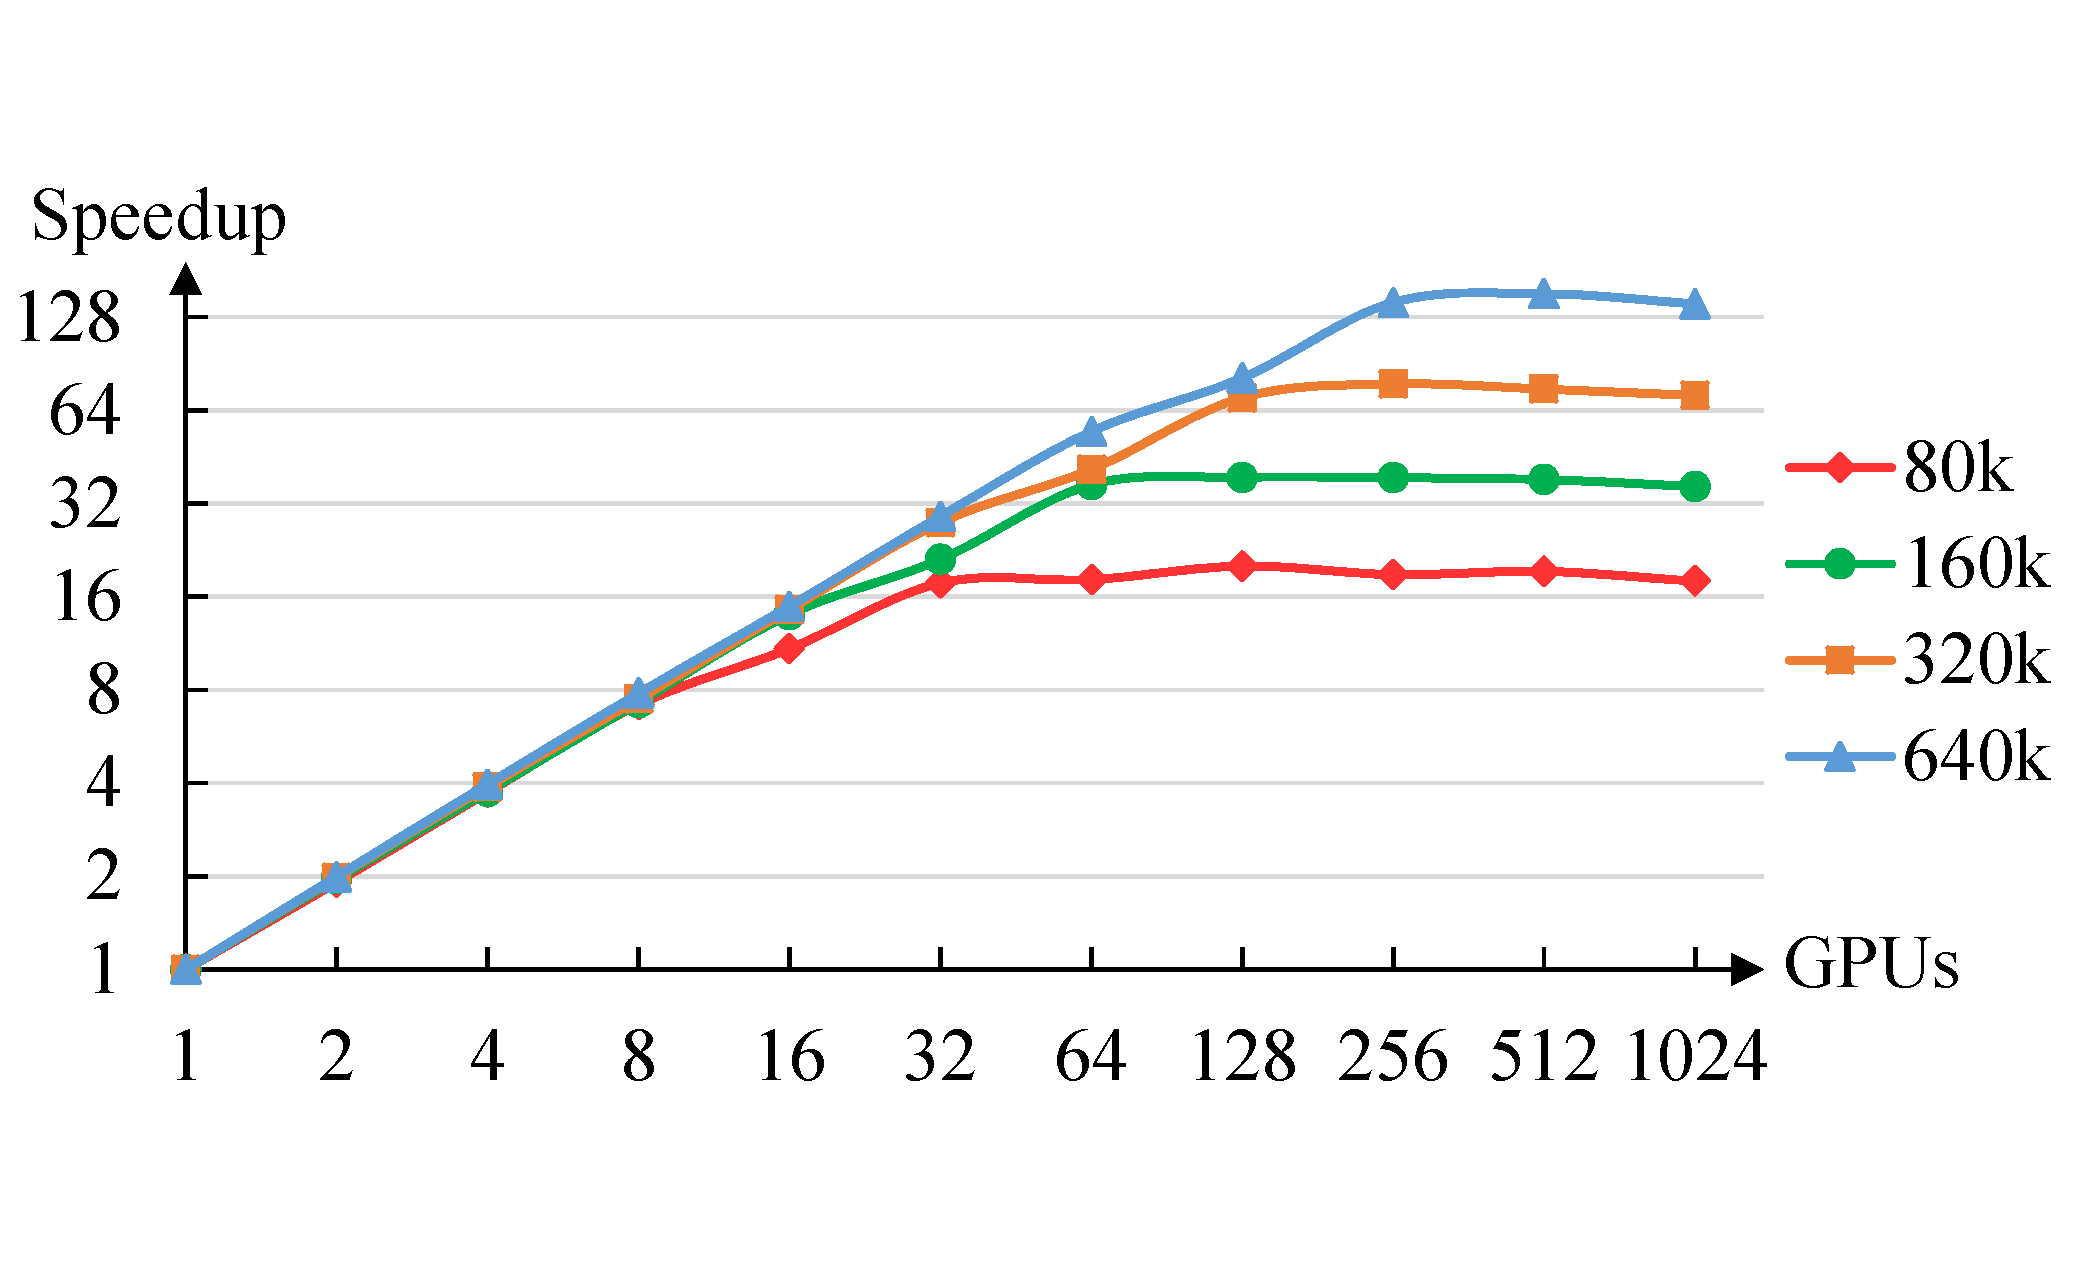
\includegraphics[width=\textwidth]{plot/640k_speedup_of_space_charge_kicker5log.pdf}
        \caption{空间电荷效应求解器加速比}
        \label{fig:SCTitan}
    \end{subfigure}
    \quad
    ~ %add desired spacing between images, e. g. ~, \quad, \qquad, \hfill etc.
      %(or a blank line to force the subfigure onto a new line)
    \begin{subfigure}[b]{0.9\textwidth}
        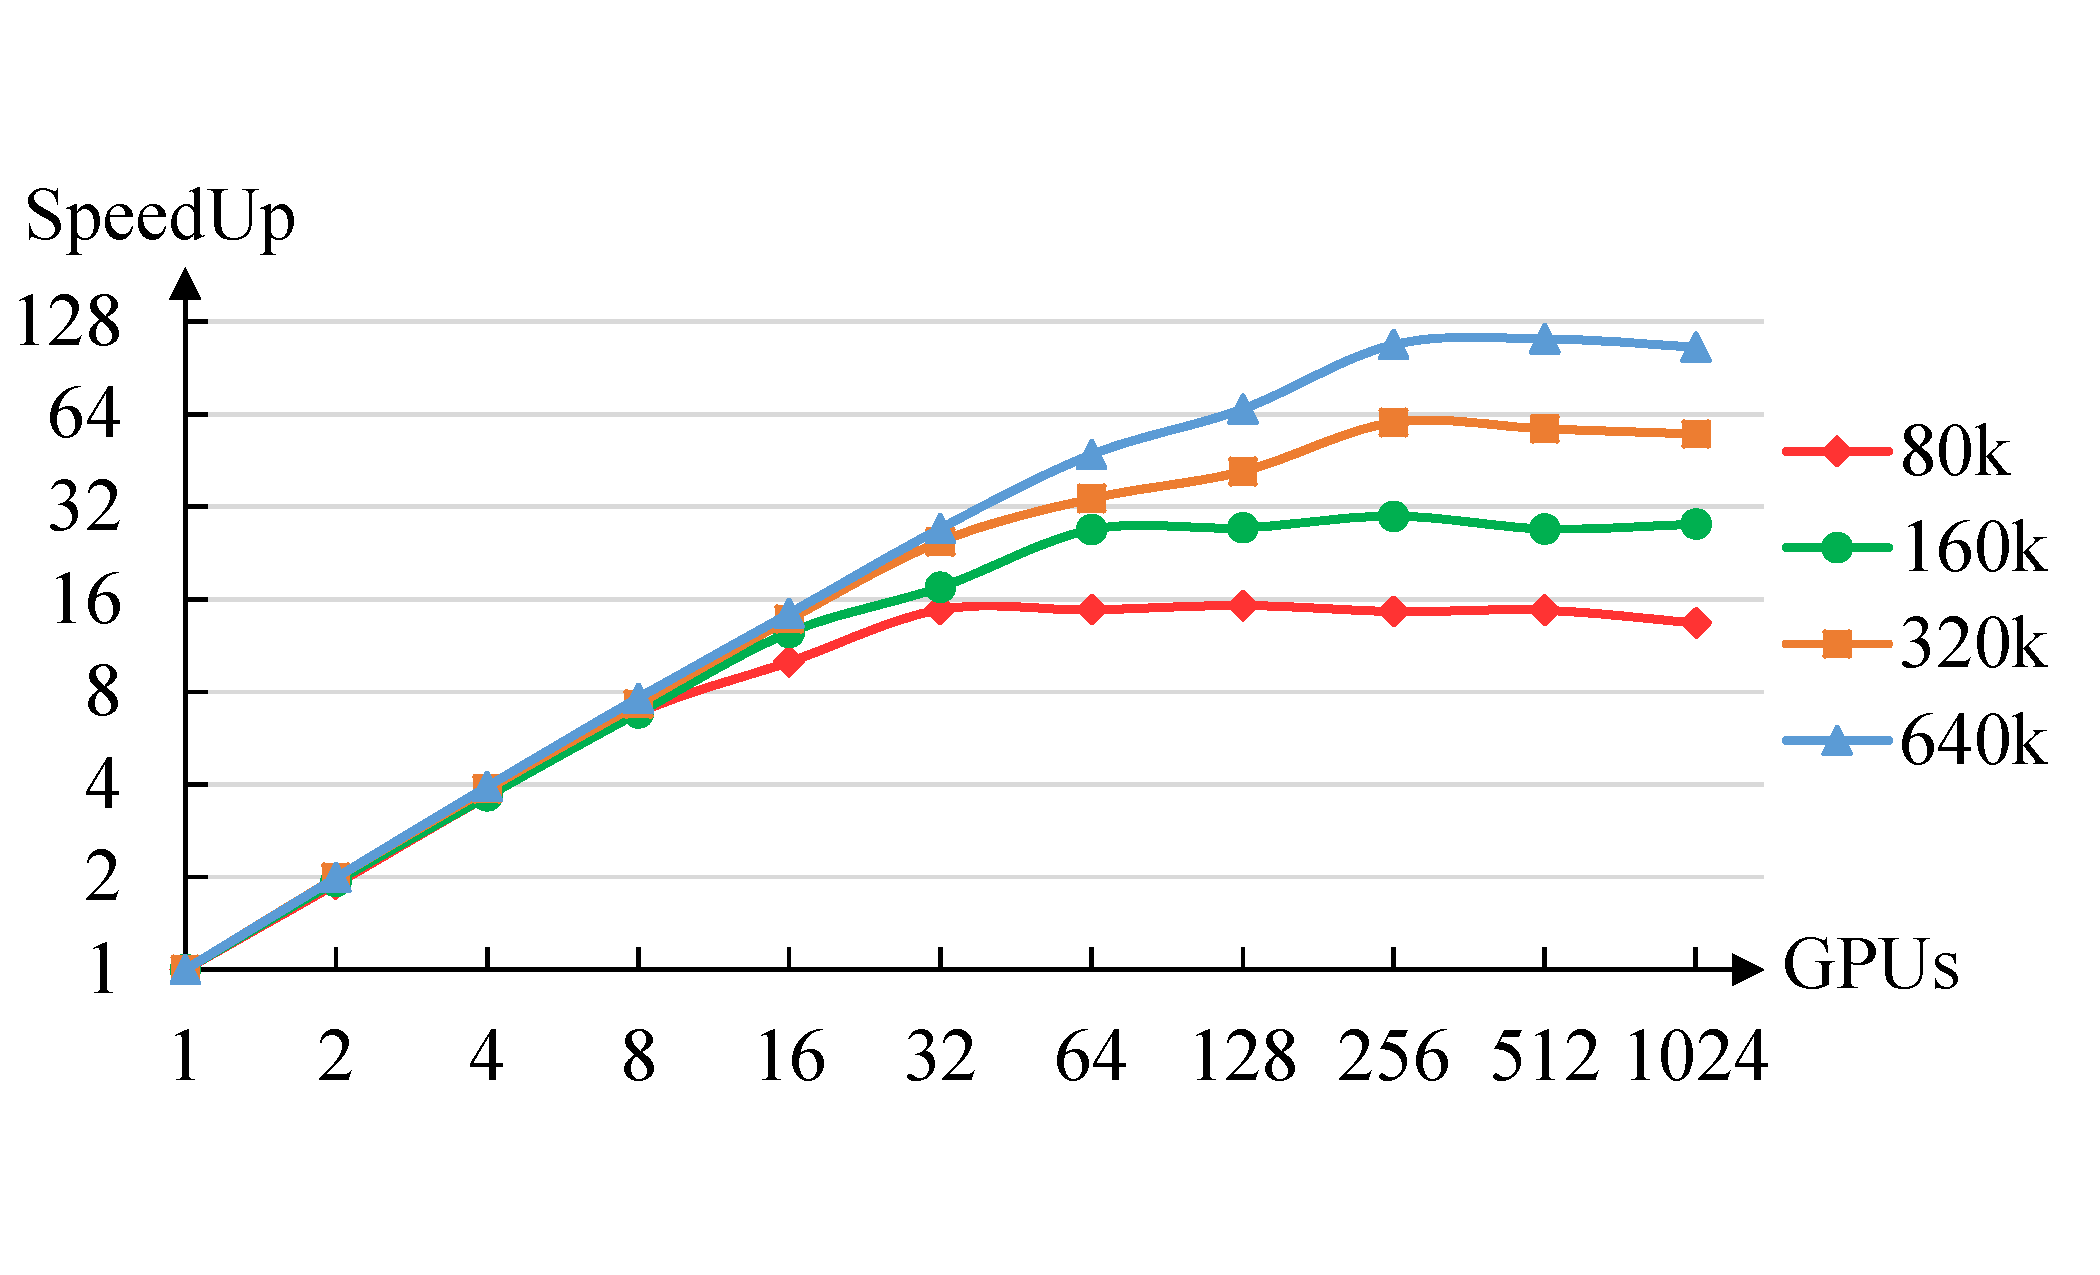
\includegraphics[width=\textwidth]{plot/640k_speedup_of_looptime5log.pdf}
        \caption{程序整体加速比}
        \label{fig:TotalTitan}
    \end{subfigure}
    \caption{多GPU加速比}\label{fig:Titan}
\end{figure}

由图\ref{fig:SCTitan}可得,在一开始,空间电荷效应求解器的加速比随着GPU的数目几乎线性增加,随后,加速比逐渐到达一个极限。
一方面,加速比的线性增长主要是因为GPU之间的数据交换量很少。这是无网格保辛粒子跟踪算法的一个很大的优势,其数据交换量仅与模式数量有关,而与粒子数量无关。
另一方面,它可以实现的最大加速度主要受粒子数量的限制,线性增加的范围和极限也随着粒子数量的增加而增加。以160000粒子为例,加速比最大可以达到40。在Titan集群上,每个GPU包含2688个内核,当使用64个GPU时,我们使用了64 $\times$ 2688 = 172032个内核,即使用的核心数多于粒子数。在这种情况下,我们无法通过简单地使用更多的GPU来获得进一步加速。而粒子数目增加时,比如320000个粒子或640000个粒子,所能够使用的GPU数目也会随之增加,最大加速比和线性范围也就会增加。

图\ref{fig:TotalTitan}是程序整体总时间的加速比,其中外部传输矩阵,坐标变换,粒子信息统计这些部分也是并行化的。但是因为它们的计算量较低,很难取得很高的并行度。所以加速比略微下降。

\section{三阶共振模拟}            \label{section:3rd_order_simulation}
我们使用这套保辛算法在周期聚焦结构中进行粒子跟踪和模拟。我们使零流强的周期相移为86.3259度,如果将10个周期视为一个环,则环的工作点为2.3979。随着流强的增加,相移会被压缩,工作点会在0.6A左右穿过2.3333的三阶共振线。环中还存在一个六极磁铁。

图\ref{fig:emitGrowthCompare}为不同流强下的束流发射度增长变化,可以看到,发射度在流强为0.1A 和0.2A 时基本保持不变,这时的工作点约为2.40。但是发射度在流强为0.4A,0.6A,和0.8A时持续增长,这时的工作点在2.3333附近,可知其发射度增长是由于三阶共振导致。

\begin{figure}[!htb]
    \centering
    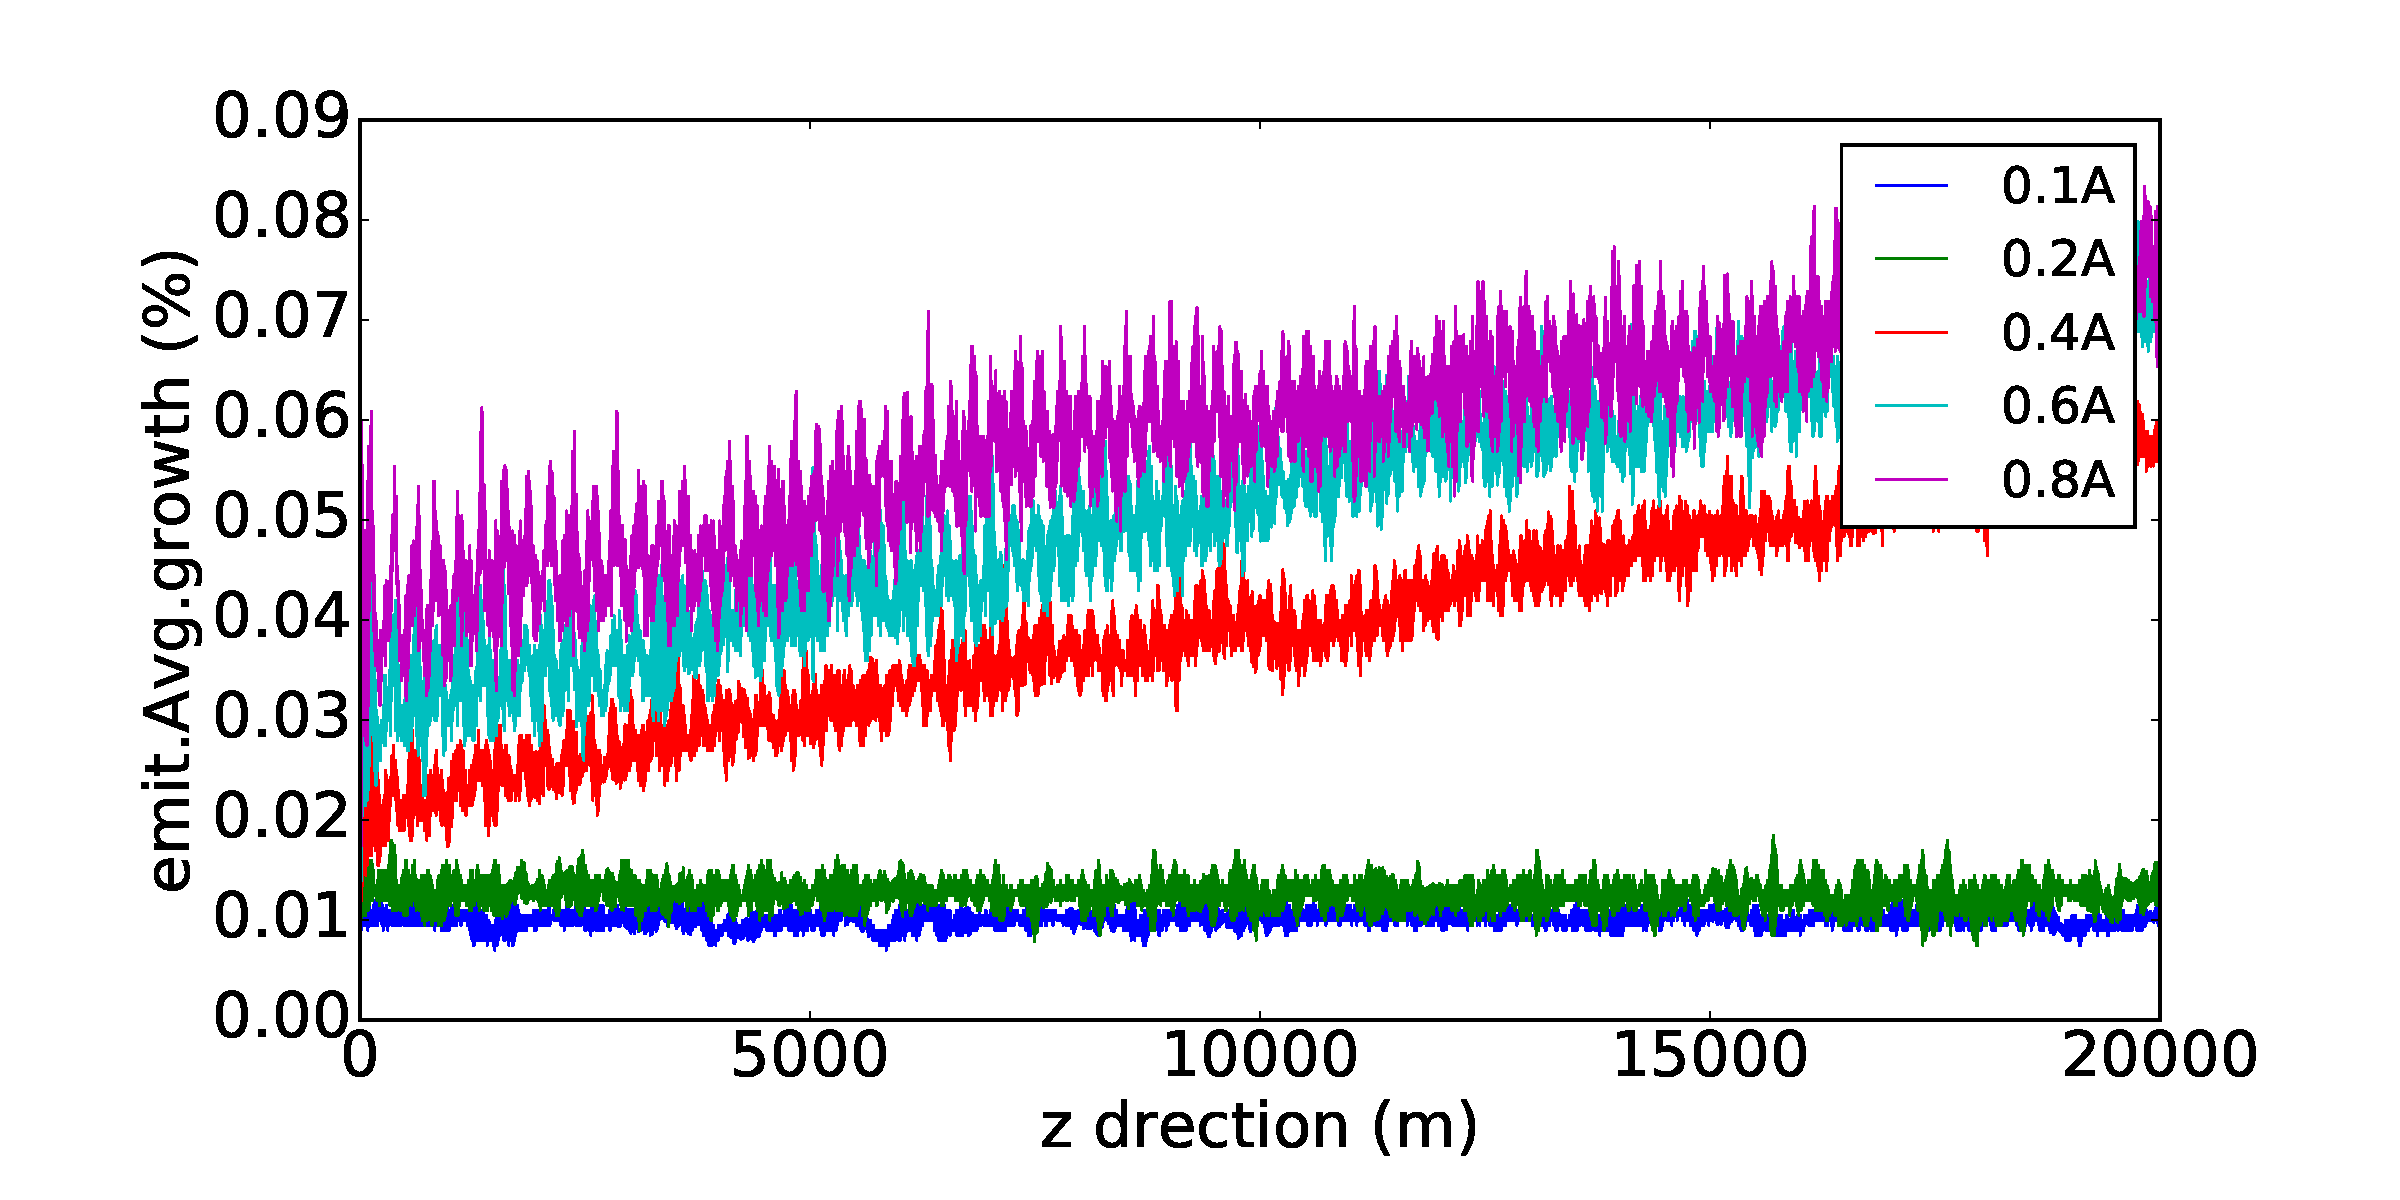
\includegraphics[width=\textwidth]{plot/emitGrowthCompare.pdf}
    \caption{不同流强下的发射度增长}
    \label{fig:emitGrowthCompare}
\end{figure}

图\ref{fig:Poincare}是工作点为2.3333附近时的粒子坐标的庞加莱截面,其中颜色越暗表示粒子密度越大,而不同的图片代表粒子处于不同的初始位置。受空间电荷效应驱动,庞加莱截面会被被扭曲,并塑造成三角形形状。受到三阶共振影响的粒子的横向位置会逐渐变大。最后,粒子会成为束晕的一部分并丢失。

\begin{figure}[!htb]
    \centering
    \begin{subfigure}[b]{0.48\textwidth}
        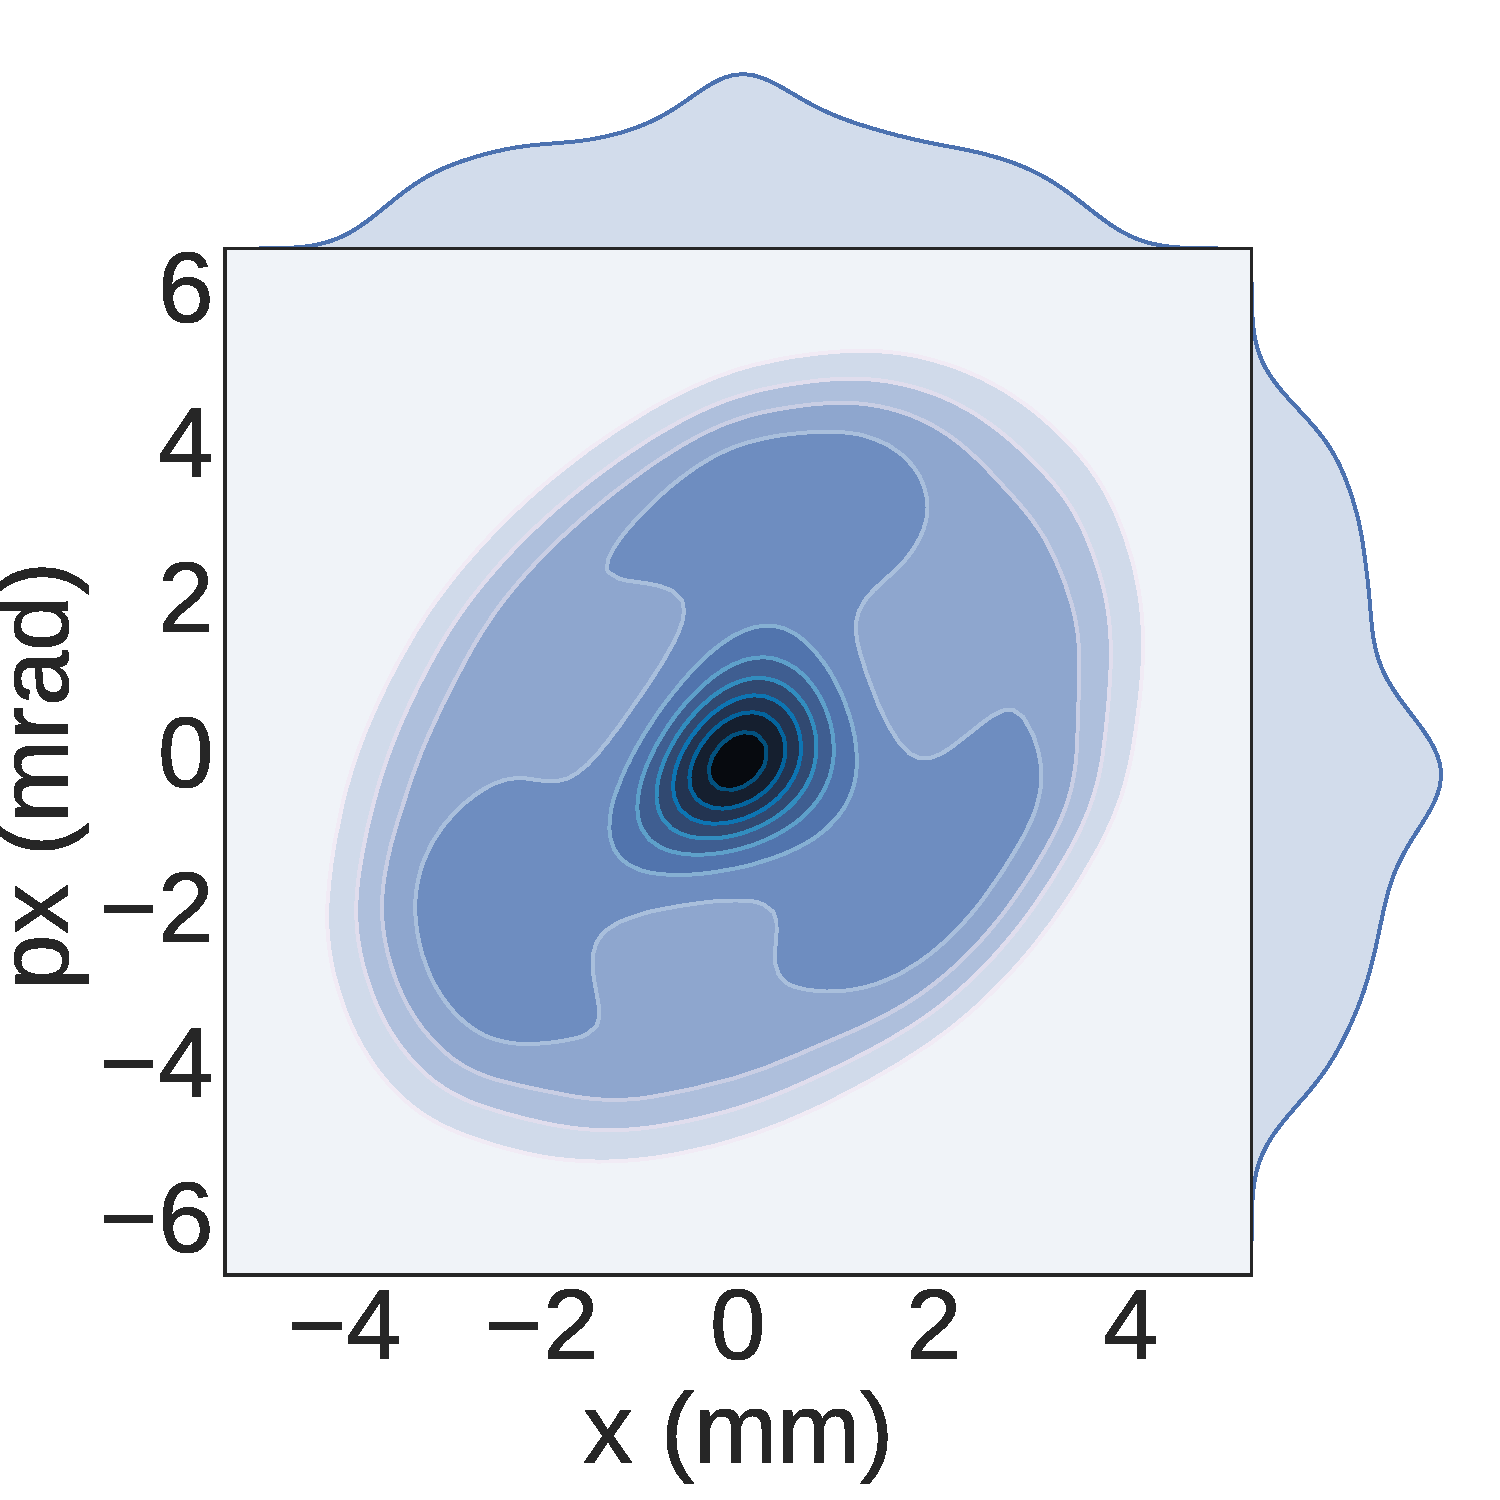
\includegraphics[width=\textwidth]{plot/particle_contour_nlevel9/sptc00002_xpx.pdf}
        \caption{}
    \end{subfigure}
    \begin{subfigure}[b]{0.48\textwidth}
        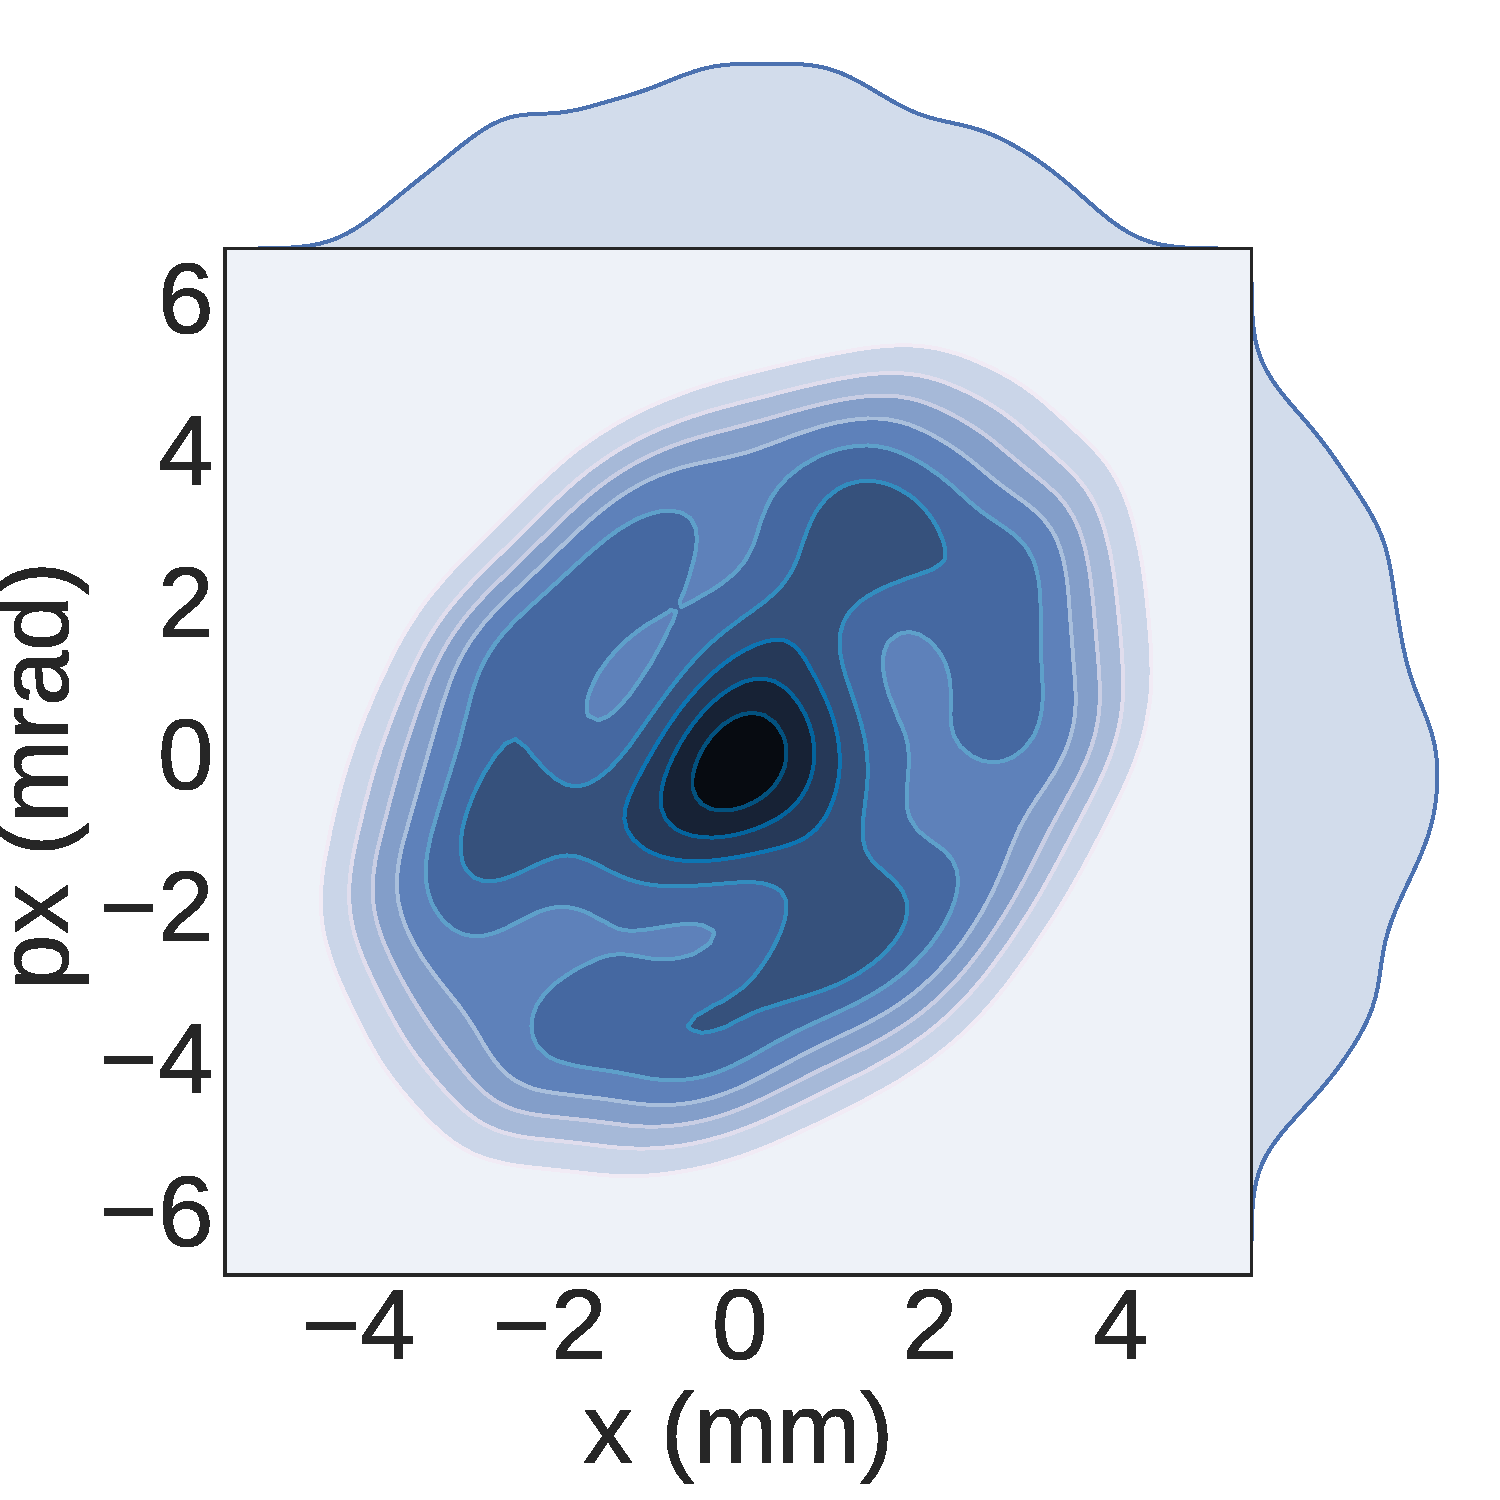
\includegraphics[width=\textwidth]{plot/particle_contour_nlevel9/sptc00005_xpx.pdf}
        \caption{}
    \end{subfigure}
    \begin{subfigure}[b]{0.48\textwidth}
        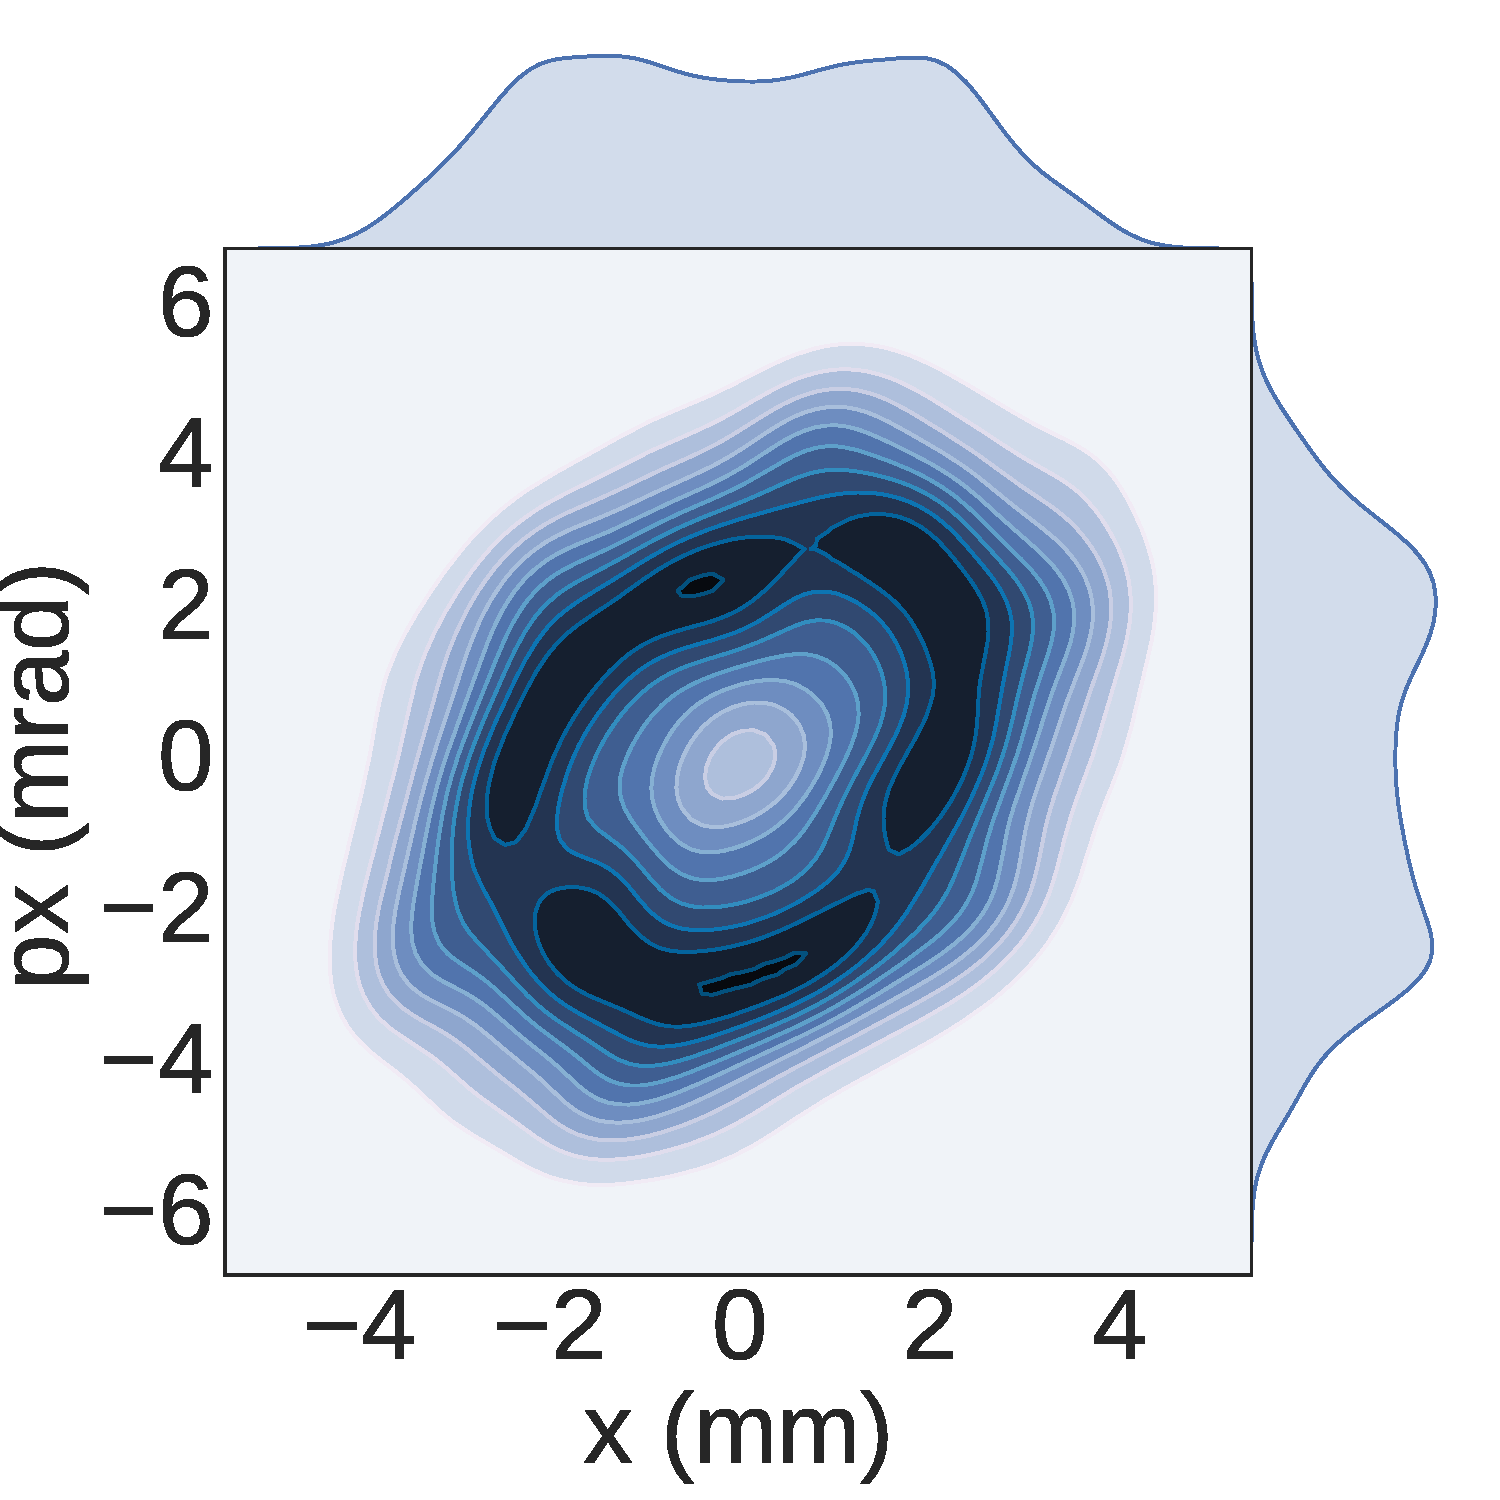
\includegraphics[width=\textwidth]{plot/particle_contour_nlevel9/sptc00003_xpx.pdf}
        \caption{}
    \end{subfigure}
    \begin{subfigure}[b]{0.48\textwidth}
        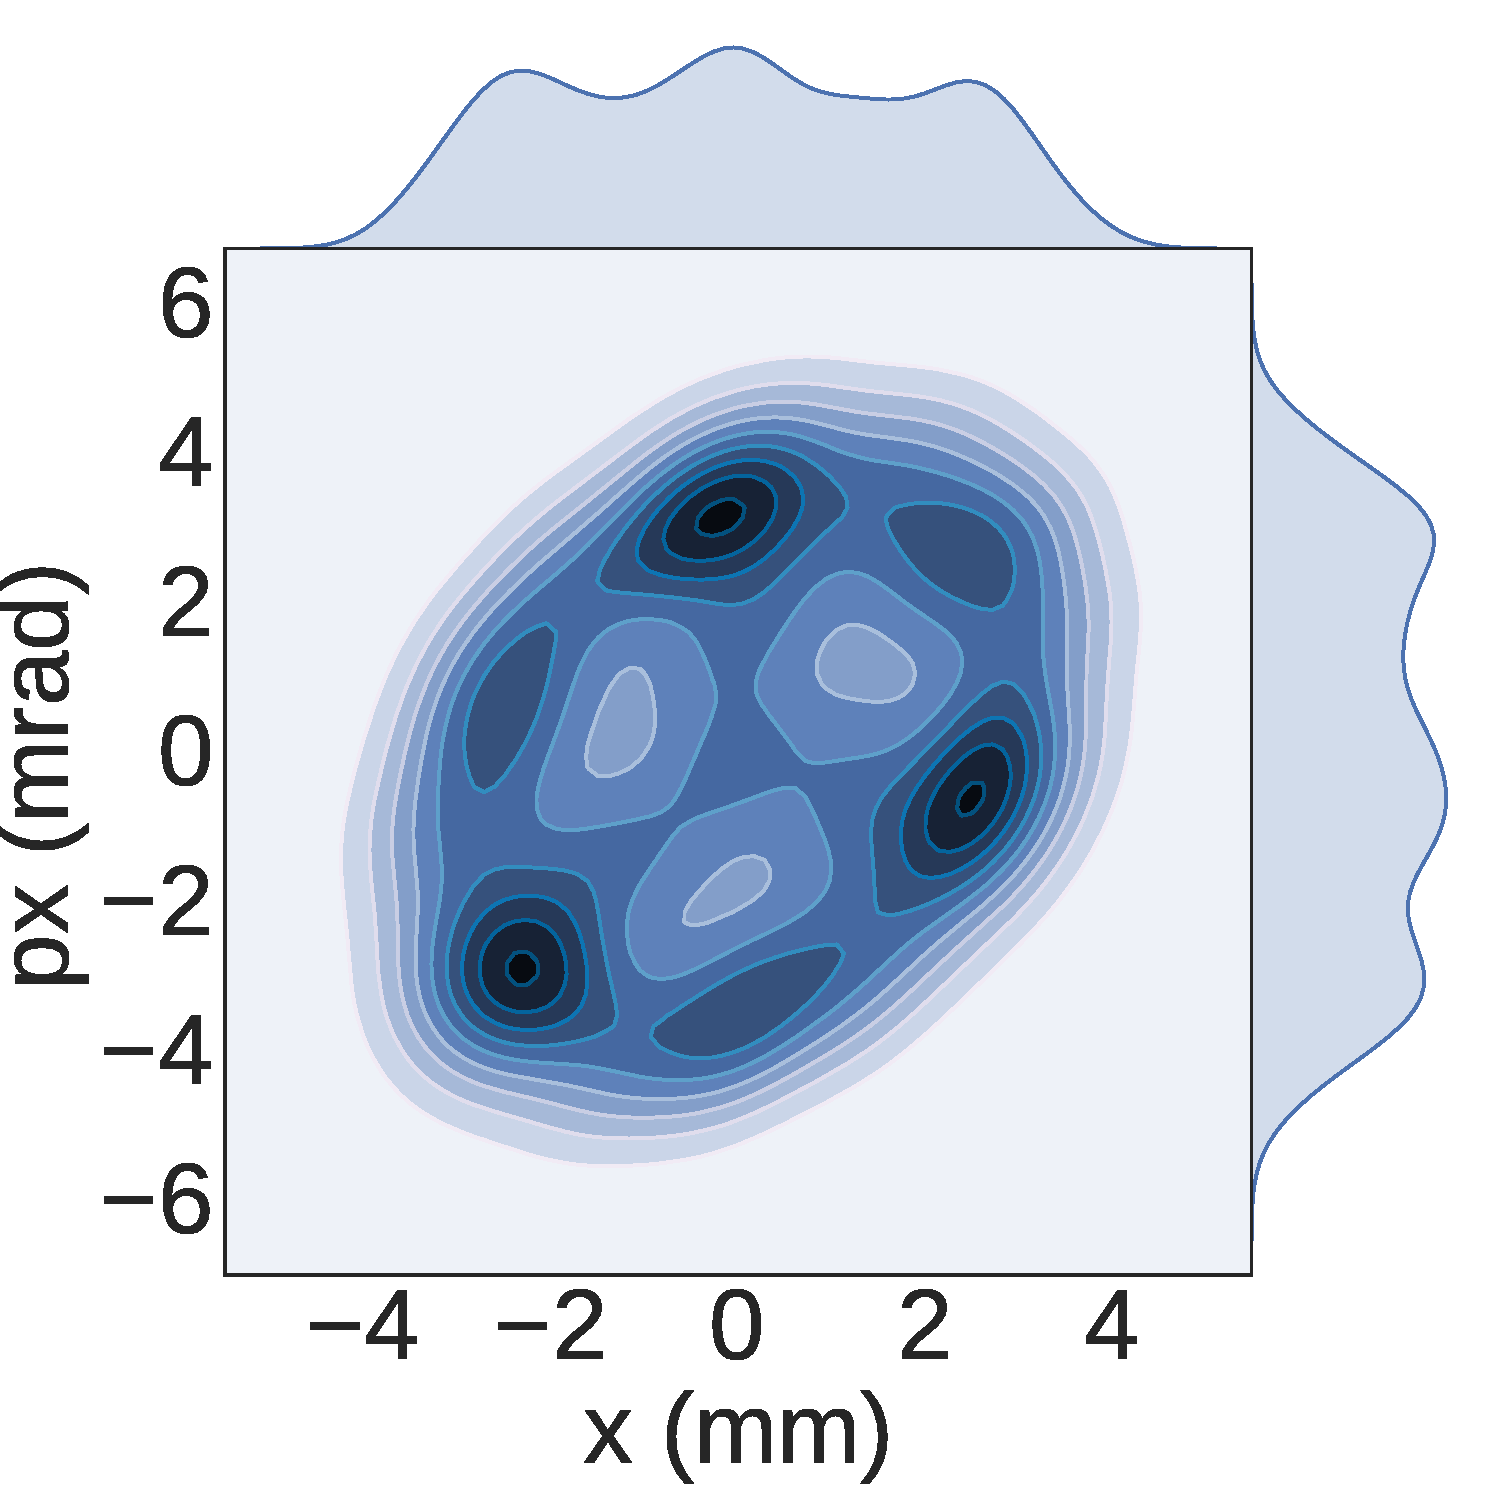
\includegraphics[width=\textwidth]{plot/particle_contour_nlevel9/sptc00006_xpx.pdf}
        \caption{}
    \end{subfigure}
    \caption{三阶共振附近的庞加莱截面}\label{fig:Poincare}
\end{figure}
\section{C-ADS注入器I模拟}        \label{section:ADS_simulation}
我们使用P-TOPO程序模拟了C-ADS的注入器I。C-ADS的注入器I由离子源(electron cyclotron resonance ion-source,ECRIS),低能传输线,RFQ,中能传输线,两个超导加速模块,以及最后的垃圾桶组成,其结构如图\ref{fig:ADS_layout}所示

\begin{figure}[!htb]
    \centering
    
\includegraphics[width=1.05\textwidth]{Img/Layout_of_ADS_Injector_I.jpg}
    \caption{C-ADS注入器I结构示意图}
    \label{fig:ADS_layout}
\end{figure}

C-ADS注入器I的基本参数如表\ref{tab:C_ADS_parameters}所示。其中RFQ是使用PARMTEQM\cite{crandall1998rfq}设计的,频率为325MHz,将10mA的质子束流从35keV加速到3.2MeV,并且以后有可能升级到15mA。因为注入能量较低,只有35keV,RFQ的参数和聚束节使用绝热设计以降低空间电荷效应的影响,这导致了最终较小的纵向发射度。RFQ之后是超导加速腔,经过14个Spoke腔将束流加速到最终的10MeV。

\begin{table}[!htbp]
    \centering
    \footnotesize% fontsize
    \setlength{\tabcolsep}{4pt}% column separation
    \renewcommand{\arraystretch}{1.2}%row space
    \begin{tabular}{lc}
        \hline\hline
        Particle                & Proton \\
        \hline
        Rf frequency (MHz)      & 325       \\
        \hline
        Injection energy (MeV)  & 0.035     \\
        \hline
        Output energy (MeV)     & 10        \\
        \hline
        Pulsed beam current (mA)& 10        \\
        \hline
        Beam duty factor        & 100\%     \\
        \hline
        Input normalized rms emittance X ($\pi$ mm mrad)    & 0.2        \\
        \hline
        Input normalized rms emittance Y ($\pi$ mm mrad)    & 0.2        \\
        \hline\hline
    \end{tabular}
    \caption{C-ADS注入器I基本参数}
    \label{tab:C_ADS_parameters}
\end{table}

我们对RFQ和后面的超导段分别进行模拟,宏粒子数目为20000个,横向初始分布使用KV分布,纵向初始分布为均匀分布。使用实际运行的加速器结构,并且当粒子的横向位置触碰元件的孔径后标记为丢失,其中RFQ稍微严格对待,其孔径为当前cell的最小半径。空间电荷效应的网格数为64*64*64(x/y/z)。在RFQ段,我们不但使用P-TOPO程序,同时也使用Track程序\cite{aseev2005track},以相同的初始条件进行模拟;同样的,在超导段,除了P-TOPO之外,我们还使用TraceWin\cite{uriot2014tracewin}来进行研究和对比。下面,我们对RFQ和超导段分别进行讨论。

\subsection{RFQ模拟}
在RFQ模拟中,RFQ中的场可由傅里叶贝塞尔方程的八项式得到,如式\ref{eq:RFQ_8terms}:
\begin{equation}
    \begin{aligned}
       {{U}_{ex}}(r,\theta ,z) & =\frac{V}{2}[{{A}_{01}}{{(r/{{r}_{0}})}^{2}}\cos (2\theta )+{{A}_{10}}{{I}_{0}}(kr)\cos (kz) \\
     & +{{A}_{03}}{{(r/{{r}_{0}})}^{6}}\cos (6\theta )+{{A}_{21}}{{I}_{2}}(2kr)\cos (2\theta )\cos (2kz) \\
     & +{{A}_{12}}{{I}_{4}}(kr)\cos (4\theta )\cos (kz)+{{A}_{03}}{{I}_{0}}(3kr)\cos (3kz) \\
     & +{{A}_{23}}{{I}_{6}}(2kr)\cos (6\theta )\cos (2kz)+{{A}_{32}}{{I}_{4}}(3kr)\cos (4\theta )\cos (3kz)]
    \end{aligned}
    \label{eq:RFQ_8terms}
\end{equation}
其中$I_n$为第n阶修正贝塞尔方程,$k=\pi /2\beta \gamma$,$A_mn$系数由RFQ设计程序PARMTEQM给出。

图\ref{fig:ADS_RFQ_emit}是P-TOPO和TRACK在0mA下和15mA下对RFQ模拟得到的横向和纵向发射度演化,其中红色实线为P-TOPO的结果而绿色虚线为TRACK的结果。在横向和纵向两个方向上,P-TOPO的发射度演变结果都更加光滑,尤其是在RFQ的前端。在此处,束流开始丝化形成束团,并且相空间开始剧烈旋转。P-TOPO与TRACK的结果误差在合理范围内。

\begin{figure}[!htb]
    \centering
    \begin{subfigure}[b]{0.9\textwidth}
        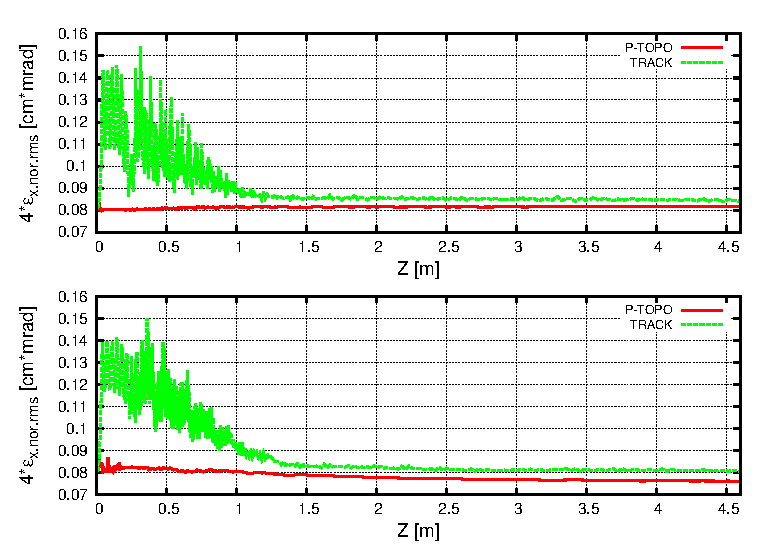
\includegraphics[width=\textwidth]{Img/ADS_RFQ_emit1.eps}
        \caption{0mA(上)和15mA(下)时RFQ中的横向发射度}
    \end{subfigure}
    \begin{subfigure}[b]{0.9\textwidth}
        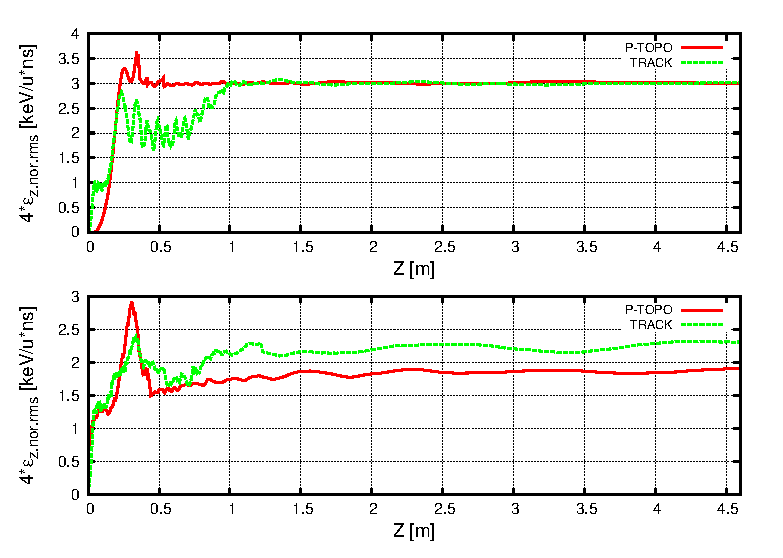
\includegraphics[width=\textwidth]{Img/ADS_RFQ_emit2.eps}
        \caption{0mA(上)和15mA(下)时RFQ中的纵向发射度}
    \end{subfigure}
    \caption{RFQ中的横向发射度和纵向发射度}\label{fig:ADS_RFQ_emit}
\end{figure}



图\ref{fig:ADS_RFQ_size1}是P-TOPO和TRACK在15mA下对RFQ模拟得到的横向束团尺寸演化,图\ref{fig:ADS_RFQ_size2}是P-TOPO和TRACK在15mA下对RFQ模拟得到的纵向束团尺寸和能散演化,其中红色实线为P-TOPO的结果而绿色虚线为TRACK的结果。两个程序在束团均方根尺寸上吻合得很好,其差别在合理范围内。同时验证了C-ADS注入器I的RFQ设计能够有效的控制束团的发射度和尺寸。

\begin{figure}[!htb]
    \centering
    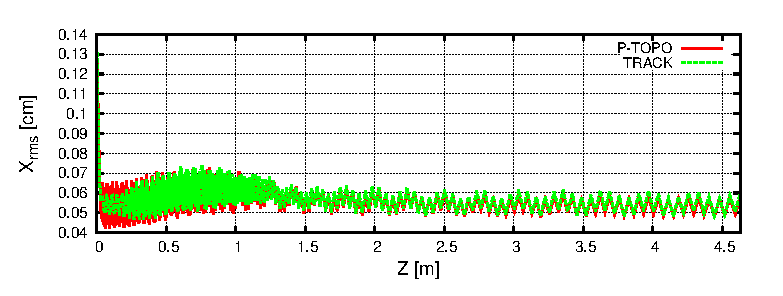
\includegraphics[width=0.9\textwidth]{Img/ADS_RFQ_size1.eps}
    \caption{RFQ中束团横向均方根尺寸}
    \label{fig:ADS_RFQ_size1}
\end{figure}

\begin{figure}[!htb]
    \centering
    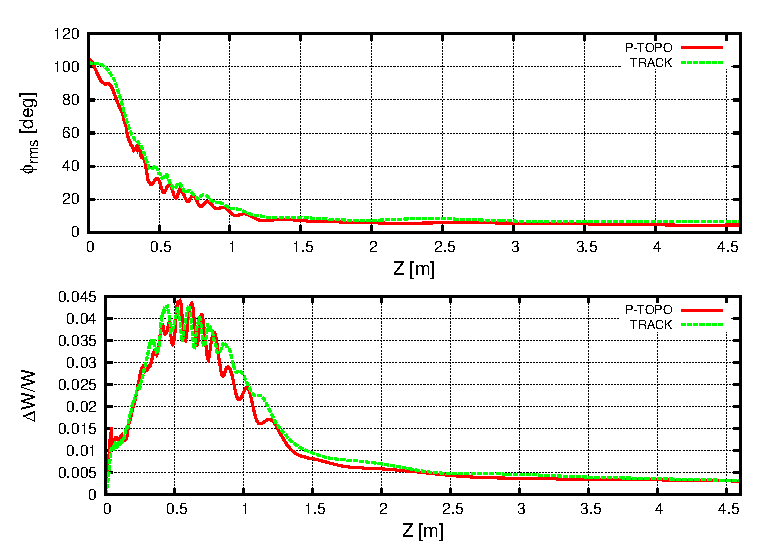
\includegraphics[width=0.9\textwidth]{Img/ADS_RFQ_size2.eps}
    \caption{RFQ中束团纵向均方根尺寸和能散}
    \label{fig:ADS_RFQ_size2}
\end{figure}

\subsection{超导段模拟}
在超导段中,聚束腔和加速腔的场由文件导入,P-TOPO使用数值差值来得到粒子所受到的场强。在设计的15mA流强下,RFQ出口处3.2MeV的质子束流经过聚束,通过MEBT进入超导段,逐渐加速到10MeV。在超导段中我们使用P-TOPO和TraceWin来进行模拟。

图\ref{fig:ADS_SC_emit}为P-TOPO和TraceWin在15mA下对RFQ模拟得到的横向和纵向发射度演化,其中红色实线为P-TOPO的结果而绿色虚线为TraceWin的结果。
两个程序得到的结果相一致。其中横向发射度除了在螺线管处有一个峰值外,基本保持不变。螺线管处的峰值是因为P-TOPO和TraceWin都是以时间t为基本变量,即发射度是由同一时刻的粒子信息统计得到,而不是由同一纵向位置的粒子得到,因此,在束团进入螺线管的时候,部分粒子先进入,部分粒子还没有进入,导致相空间的扭曲,从而导致统计发射度的突变。纵向发射度有略微增长,增长幅度在20\%以内。横纵向的发射度增长是由空间电荷力,磁铁边缘场的非线性效应,以及超导腔内的非线性纵向力导致,这几个驱动发射度增长的来源共同作用,使粒子相空间扭曲,最终会导致束晕的产生。P-TOPO的模拟中,出口能量为10.01MeV,而TraceWin的模拟出口能量为10.06MeV。
\begin{figure}[!htb]
    \centering
    \begin{subfigure}[b]{0.9\textwidth}
        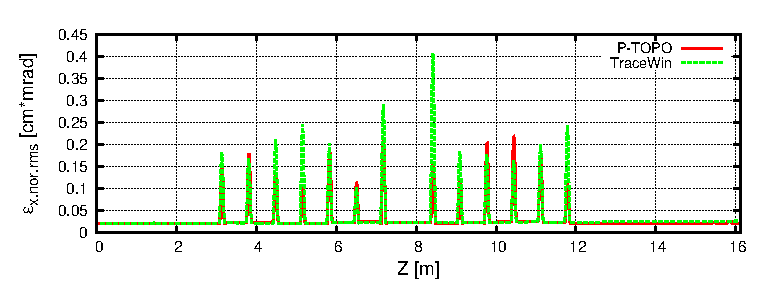
\includegraphics[width=\textwidth]{Img/ADS_SC_emit1.eps}
        %\caption{}
    \end{subfigure}
    \begin{subfigure}[b]{0.9\textwidth}
        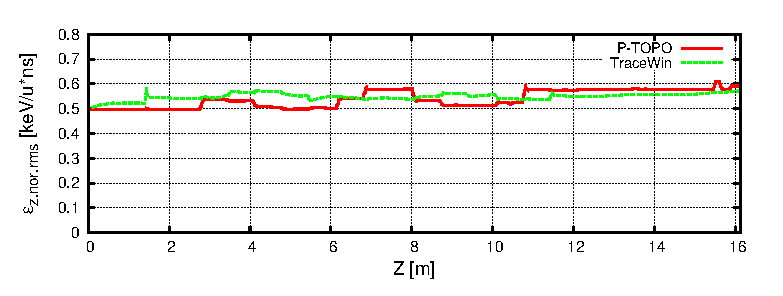
\includegraphics[width=\textwidth]{Img/ADS_SC_emit2.eps}
        %\caption{}
    \end{subfigure}
    \caption{超导段横向发射度和纵向发射度}\label{fig:ADS_SC_emit}
\end{figure}

图\ref{fig:ADS_SC_size}是P-TOPO和TraceWin在15mA下对超导段模拟得到的横纵向束团尺寸演化和能散演化,其中红色实线为P-TOPO的结果而绿色虚线为TRACK的结果。两个程序模拟结果的细微差别主要是因为两个程序获取同步相位的方法不同。TraceWin使用时间漂移法获得同步相位,而P-TOPO使用扫相获得同步相位。束团的横向尺寸相比管道半径都很小,而纵向尺寸也被聚束腔和接下来的各个加速腔有效地压缩,一般不会有束损出现。
\begin{figure}[!htb]
    \centering
    \begin{subfigure}[b]{0.9\textwidth}
        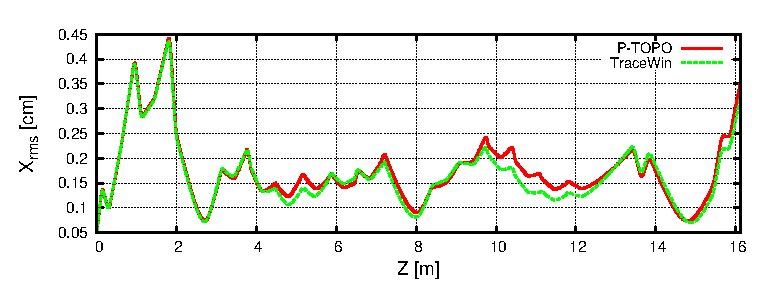
\includegraphics[width=\textwidth]{Img/ADS_SC_size1.eps}
        %\caption{}
    \end{subfigure}
    \begin{subfigure}[b]{0.9\textwidth}
        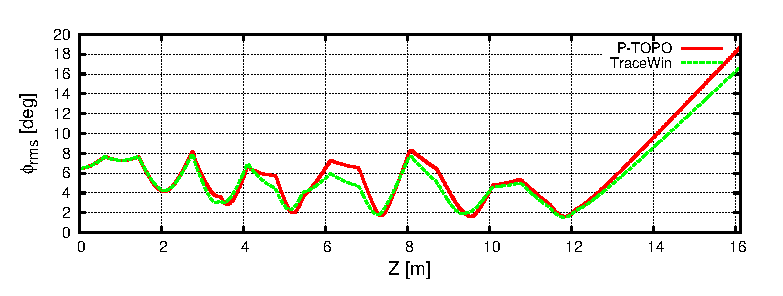
\includegraphics[width=\textwidth]{Img/ADS_SC_size2.eps}
        %\caption{}
    \end{subfigure}
    \begin{subfigure}[b]{0.9\textwidth}
        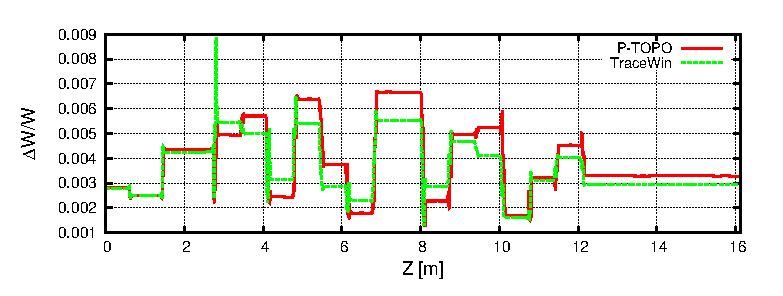
\includegraphics[width=\textwidth]{Img/ADS_SC_size3.eps}
        %\caption{}
    \end{subfigure}
    \caption{超导段束团横纵向尺寸以及能散}\label{fig:ADS_SC_size}
\end{figure}

在RFQ和超导段两段模拟中,传输效率都在99.9\%以上,束团尺寸和束损都得到了有效控制,横向和纵向的发射度都保持良好。不同代码的模拟结果差别主要是因为初始的束团分布不同,以及统计数据的方式不同,特别是P-TOPO是以时间t为基本变量,而TRACK是以位置z为基本变量,因此粒子信息收集,空间电荷力的计算,以及粒子推动方式都有所不同。

\section{小结}                    \label{section:Simulation_conclusion}
通过对并行程序的性能测试可以看出,对于PIC算法在单个普通家用GPU(GTX 1060)上相对于单核CPU实现了超过50倍的加速。
当模拟使用的粒子数较大时,PIC算法在GPU集群上也显示出良好的可扩展性;而当粒子数目较小时其可扩展性较差。

对于Symplectic算法,在一个普通家用GPU上相对于单核CPU实现了接近500倍的加速比。
同时,我们在GPU集群泰坦上的测试还显示出这种算法有良好的可扩展性,程序的加速比随着GPU数目几乎线性增加。

我们在周期性聚焦结构中使用Symplectic算法进行了几个应用模拟,当工作点远离共振线时,束流不会出现发射度增长,而当其接近共振线时发射度会持续增长。
在未来的研究中,我们将继续扩展此模型速发,并在不同架构的计算机上比较保辛算法的效率。

最后,我们使用P-TOPO程序对C-ADS注入器I的RFQ和超导段分别进行了模拟并且与其他程序进行了比较。
模拟结果证明了现有设计的合理性,束团的尺寸和发射度都得到了有效控制,束损以及能散也在合理范围之内,完全满足需求。
之后,我们将继续对P-TOPO进行拓展并加入更多新的功能,以满足强流加速器的各种需求。